\documentclass[conference]{IEEEtran}
\IEEEoverridecommandlockouts

\usepackage{cite}
\usepackage{amsmath,amssymb,amsfonts}
\usepackage{algorithmicx}
\usepackage{algpseudocode}
\usepackage{graphicx}
\usepackage{textcomp}
\usepackage{xcolor}
\usepackage{listings} % Added for Haskell formatting
\usepackage{float}
\usepackage{algorithm}
\usepackage{booktabs}
\usepackage{multirow}
\usepackage{microtype}
\usepackage{url}

\def\BibTeX{{\rm B\kern-.05em{\sc i\kern-.025em b}\kern-.08em
    T\kern-.1667em\lower.7ex\hbox{E}\kern-.125emX}}

\begin{document}

\title{Synthesising the Aperture: A Comparative Study of Heuristic Search Methods for Radio Astronomy}

\author{\IEEEauthorblockN{J.M. Ward}
\IEEEauthorblockA{\textit{Computer Science Department} \\
\textit{Stellenbosch University}\\
Stellenbosch, South Africa \\
24913707@sun.ac.za
}
}

\maketitle
\thispagestyle{plain}
\pagestyle{plain}

\begin{abstract}
The design of radio interferometer arrays presents a massive non-convex combinatorial optimisation problem. 
This study investigates the discrete selection of a 16-antenna subset from the 64-pad MeerKAT array, aiming to 
maximise central $uv$-coverage density for high-fidelity image reconstruction. A trajectory-based Simulated 
Annealing (SA) algorithm was empirically compared against four configurations of a population-based Genetic 
Algorithm (GA) utilising a Gaussian-weighted spatial frequency objective function. Results across 30 independent 
executions demonstrate that SA significantly outperforms all evolutionary variants ($p = 1.88445 \times 10^{-11}$). 
Topographic analysis reveals that SA successfully isolated a centrally clustered antenna geometry that perfectly 
aligned with the weighted objective. Conversely, the GA configurations suffered from premature convergence, as the 
intersection crossover operator proved destructive to high-fitness spatial neighbourhood traits. These findings 
establish the superiority of targeted, thermodynamic trajectory search over standard evolutionary recombination 
for the discrete aperture synthesis problem.
\end{abstract}

\section{Introduction}

The introduction section establishes the context of the radio antenna placement problem. 
The section defines the core objectives of the study and provides an outline for the remainder of the report.

Radio interferometry enables high-resolution celestial imaging by combining signals 
from an array of individual antennas~\cite{thompson2017}. The quality of the synthesized image depends heavily 
on the physical configuration of the participating antennas. An optimal arrangement maximises 
spatial frequency sampling and minimises noise artefacts in the resulting observations. 
Therefore, the design of the antenna layout is a critical component of modern astronomical architecture.

The MeerKAT radio telescope presents a complex configuration challenge. The MeerKAT array 
consists of 64 available physical ground pads. Observational and processing constraints often 
mandate the selection of a subset of 16 active antennas for specific imaging tasks. 
The primary objective is to identify a geometric layout that maximises the density of 
the $uv$-coverage to ensure high-fidelity image reconstruction. 

Selection of the optimal 16 antennas from the 64 available pads yields a search space of 
approximately $4.88 \times 10^{14}$ distinct combinations. Exhaustive mathematical evaluation 
of every combination requires prohibitive computational resources. Consequently, advanced 
heuristic search techniques are necessary to identify optimal or near-optimal configurations 
within a feasible timeframe. 

The purpose of the study is to evaluate the efficacy of computational intelligence metaheuristics 
applied to the antenna placement problem. Specifically, a baseline genetic algorithm, 
three distinct genetic algorithm variants, and a simulated annealing algorithm were 
implemented and tested. The genetic algorithm variants investigated the impact of adjusting 
selection pressure, diversity maintenance, and mutation rates on the evolutionary search process. 
Simulated annealing employed a trajectory-based thermodynamic model to refine a single configuration. 
The empirical performance of the algorithmic variants was compared to determine the most effective 
search strategy for $uv$-coverage optimisation.

Empirical results across 30 independent executions demonstrate that simulated annealing 
significantly outperformed all evolutionary configurations. The thermodynamic search 
discovered a centrally clustered antenna geometry that the crossover-based recombination 
operator was structurally unable to produce, establishing the superiority of trajectory-based 
exploitation for this discrete, Gaussian-weighted optimisation problem.

The remainder of the document is structured as follows. Section 2 provides the theoretical 
background of radio interferometry and defines the metaheuristic search algorithms. Section 3 
details the methodology and structural design used to implement the algorithms. Section 4 
describes the empirical procedure and parameter configurations followed during experimentation. 
Section 5 presents the research results and convergence analysis. Finally, Section 6 summarises 
the findings and concludes the report.

The following section establishes the theoretical foundation of radio interferometry and 
the metaheuristic methods applied to the optimisation problem.
\section{Background}

The background section provides the theoretical context and outline for the remainder of the discussion. 
The section begins with the physical principles of radio interferometry and aperture synthesis. 
The narrative subsequently details the spatial frequency domain and the impact of visibility sampling 
on image fidelity. Furthermore, the combinatorial complexity of antenna placement is formalised. 
Finally, the section introduces the metaheuristic search methods applied to solve the antenna 
placement optimisation problem.

\subsection{Principles of Radio Interferometry}
The angular resolution, $\theta$, of a single-dish radio telescope is fundamentally constrained 
by the diffraction limit. The diffraction limit is defined as $\theta \approx \frac{\lambda}{D}$, 
where $\lambda$ is the observation wavelength and $D$ is the aperture diameter. To capture high-resolution 
images at radio wavelengths, a single dish requires a diameter spanning several kilometres. Construction of 
a telescope of such magnitude is an engineering impossibility~\cite{thompson2017}.

Interferometry bypasses the physical limitation through aperture synthesis. By correlating the signals 
received by an array of smaller and widely spaced antennas, a virtual telescope is created. 
The virtual telescope possesses an effective diameter equal to the maximum physical separation 
distance between the antenna elements. The mathematical foundation of aperture synthesis is the Van 
Cittert-Zernike theorem. The theorem states that the complex visibility function, $V(u,v)$, measured 
by a baseline and the brightness distribution of the sky, $I(l,m)$, form a Fourier pair. A baseline is 
defined as the geometric vector connecting any pair of antennas~\cite{thompson2017}.

\subsection{The $uv$-Plane and Image Fidelity}
The spatial frequencies sampled by the baselines are mapped onto a two-dimensional coordinate system 
known as the $uv$-plane~\cite{thompson2017}. Earth Rotation Aperture Synthesis, abbreviated as ERAS, is the phenomenon 
where the rotation of the Earth continuously shifts the orientation of the physical baselines relative 
to the celestial source. The geometric shifting traces elliptical tracks in the spatial frequency 
domain over the observation period. 

The critical nature of the antenna layout problem lies in the resulting sampling distribution. 
Every unsampled region in the $uv$-plane corresponds to missing spatial information in the final 
reconstructed image. Missing information leads to noise artefacts known as sidelobes in the Point 
Spread Function, abbreviated as PSF. An optimal antenna layout maximises the density of the $uv$-coverage. 
Maximum density ensures high-fidelity reconstructions that effectively distinguish faint astronomical 
structures from instrumental noise.

Figure 1 illustrates the spatial frequency coverage generated by 
the complete 64-antenna MeerKAT 
array\footnote{\url{https://skaafrica.atlassian.net/wiki/spaces/ESDKB/pages/277315585/MeerKAT+specifications\#uv-coverage}}. 
The complete array produces a highly dense central sampling region. The empirical optimisation of the 16-antenna subset aims 
to mathematically approximate the dense core demonstrated by the full configuration.

\begin{figure}[htbp]
    \centering
    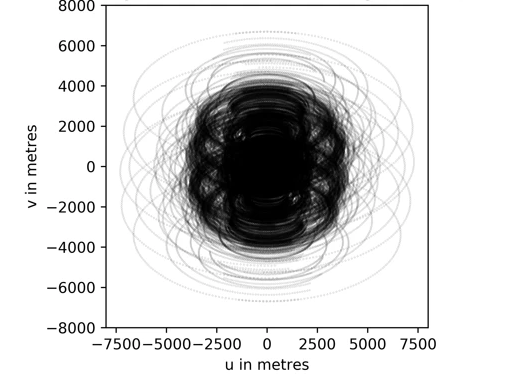
\includegraphics[width=0.8\linewidth]{meerKatUV.png}
    \caption{Simulated $uv$-coverage for the complete 64-antenna MeerKAT array.}
    \label{fig:meerkat_uv_full}
\end{figure}

\subsection{Optimisation Complexity}
Determination of the optimal placement of antennas within a fixed geographic area is a non-convex 
combinatorial optimisation problem characterised by an immense search space. For a configuration 
utilising a specific number of active antennas, $k$, selected from a total number of available 
physical pads, $n$, the number of unique combinations, $C$, is formalised as
\begin{equation}
C(n, k) = \binom{n}{k} = \frac{n!}{k!(n-k)!}.
\end{equation}
In the context of the MeerKAT array, selecting $k = 16$ active antennas out of $n = 64$ available 
physical pads yields a search space of
\begin{equation}
C(64, 16) = \binom{64}{16} \approx 4.88 \times 10^{14} \text{ configurations}.
\end{equation}

Evaluation of each candidate layout requires simulation of baseline tracks over an eight-hour observation 
window and execution of grid-based density calculations. Therefore, an exhaustive search of the configuration 
space is computationally prohibitive~\cite{engelbrecht2007}. The high computational cost necessitates the use of 
metaheuristics to balance the exploration of the vast combinatorial space with the exploitation of 
high-fitness local regions~\cite{engelbrecht2007}.

\subsection{Computational Intelligence Metaheuristics}
The combinatorial explosion of the antenna placement problem requires advanced search 
techniques. Two prevalent metaheuristics applied to the domain are genetic algorithms 
and simulated annealing. Population-based methods maintain a set of candidate solutions 
and use selection and recombination to propagate fit traits across successive generations, 
enabling simultaneous exploration of multiple regions of the search landscape. 
Trajectory-based methods instead track a single candidate solution and employ stochastic 
acceptance criteria to escape local optima that would trap traditional hill-climbing 
approaches. The two paradigms represent fundamentally different strategies for navigating 
the exploration-exploitation trade-off inherent to all combinatorial optimisation problems~\cite{engelbrecht2007}.

\subsection{Review of Current Literature}
The optimisation of radio interferometry arrays is a well-documented challenge in 
astronomical literature. Prior work has addressed the antenna placement problem using continuous optimisation 
techniques, including particle swarm optimisation and standard evolutionary algorithms 
applied to Very Long Baseline Interferometry networks~\cite{thompson2017}. The majority 
of this literature permits antennas to occupy arbitrary geographical coordinates rather 
than a fixed discrete grid.

The current empirical study differs from the established literature by framing the 
optimisation strictly as a discrete subset selection problem. The physical 
infrastructure of the MeerKAT observatory restricts antenna placement to a fixed 
grid of 64 pre-constructed pads. Therefore, the algorithm must select exactly 16 
discrete locations rather than generating continuous coordinates. Furthermore, the 
current study explicitly investigates the application of fitness sharing mechanisms. 
The literature rarely addresses the specific use of diversity maintenance to navigate 
the highly deceptive, discrete search landscape of the MeerKAT $uv$-plane.

\subsection{Justification of Metaheuristic Selection}
The discrete combinatorial explosion of the subset selection problem renders traditional deterministic 
search methods computationally unfeasible. The immense, non-convex search space requires advanced heuristic 
techniques capable of balancing global exploration with local exploitation.

The genetic algorithm was selected as the primary metaheuristic to solve the optimisation problem. 
The population-based architecture of the genetic algorithm provides robust global exploration capabilities 
across rugged fitness topographies. Maintaining a diverse population allows the algorithm to evaluate multiple 
promising regions of the $uv$-plane simultaneously. 

Simulated annealing was selected as the secondary metaheuristic to provide a comparative trajectory-based 
baseline. Simulated annealing explores the search landscape by tracking a single solution. 
The algorithm utilises the Metropolis criterion to stochastically accept inferior solutions 
early in the search process. The acceptance of inferior solutions provides a mathematically proven mechanism 
to escape local optima. Comparison of the population-based genetic algorithm against the trajectory-based 
simulated annealing provides a comprehensive evaluation of search strategies for discrete aperture synthesis 
optimisation.

\subsubsection{Genetic Algorithms}
A genetic algorithm, abbreviated as GA, is a population-based search technique inspired by Darwinian evolution~\cite{engelbrecht2007}. In the context of array design, the GA maintains a diverse pool of candidate layouts. A diverse pool allows fit genetic traits, specifically high-performing antenna pairings, to propagate through successive generations via recombination~\cite{bremermann1962}. To prevent premature convergence on local optima, a fitness sharing mechanism is utilised to penalise candidate solutions that are spatially similar. This enforces population diversity. Furthermore, an elitism mechanism guarantees the survival of the highest-performing layout across generations. The procedural flow of the GA is outlined in Algorithm 1.

\begin{algorithm}[htbp]
\caption{Genetic Algorithm incorporating fitness sharing, intersection crossover, and elitism.}
\begin{algorithmic}[1]
\State Initialise the population with a defined number of random candidate configurations
\State Ensure each candidate configuration contains exactly the required number of active antennas
\While{the termination criteria are not met}
    \State Evaluate the raw fitness of each configuration using the weighted $uv$-density
    \State Identify the configuration with the highest raw fitness to serve as the elite individual
    \State Adjust the raw fitness of each configuration using a fitness sharing penalty based on the niche radius
    \State Create an empty population for the new generation
    \State Add the elite individual directly to the new generation population
    \While{the new generation population is not full}
        \State Select two parent configurations using tournament selection based on the adjusted fitness
        \State Apply intersection crossover to the parents to generate a single child configuration
        \State Apply mutation by probabilistically swapping active antennas with inactive pads
        \State Add the mutated child configuration to the new generation population
    \EndWhile
    \State Replace the current population with the new generation population
\EndWhile
\State Return the elite individual
\end{algorithmic}
\end{algorithm}

\subsubsection{Simulated Annealing}
Simulated annealing, abbreviated as SA, is a trajectory-based metaheuristic modelled after 
the thermodynamic cooling of metals~\cite{engelbrecht2007}. The SA algorithm explores the search landscape 
by tracking a single solution and utilising the Metropolis criterion to stochastically accept 
inferior solutions early in the search. Acceptance of inferior solutions provides a vital 
mechanism to escape local optima that typically trap traditional hill-climbing methods~\cite{engelbrecht2007}. 
The procedural flow of the SA is outlined in Algorithm 2.

\begin{algorithm}[htbp]
\caption{Simulated Annealing utilising a geometric cooling schedule.}
\begin{algorithmic}[1]
\State Generate a random candidate configuration to serve as the current solution
\State Ensure the configuration contains exactly the required number of active antennas
\State Assign a high initial temperature to the system
\While{the system temperature is greater than the minimum threshold}
    \State Generate a neighbour configuration by swapping one active antenna with an inactive pad
    \State Calculate the change in fitness between the neighbour configuration and the current solution
    \If{the neighbour configuration improves the fitness or satisfies the Metropolis criterion}
        \State Accept the neighbour configuration as the new current solution
    \EndIf
    \State Reduce the system temperature according to a geometric cooling multiplier
\EndWhile
\State Return the current solution
\end{algorithmic}
\end{algorithm}

The following section details the specific implementation of the objective function, the 
simulated annealing baseline, and the four genetic algorithm configurations evaluated 
during the empirical study.
\section{Methodology}

The methodology section details the structural design and configuration of the metaheuristic algorithms evaluated during the 
empirical study. The section defines the objective function used to evaluate candidate solutions. Furthermore, the Simulated 
Annealing configuration implemented as a baseline trajectory comparator is described. Finally, the section outlines the specific 
variations applied to the genetic algorithm to analyse the impact of selection pressure, diversity maintenance, and mutation rates 
on the discrete subset selection problem.

\subsection{Objective Function Evaluation}
The primary metric for evaluating candidate configurations was a weighted $uv$-coverage density score. 
The evaluation algorithm generated geometric baseline vectors for a given 16-antenna layout. 
The evaluation algorithm projected the baseline vectors onto a two-dimensional spatial frequency grid. 
The spatial frequency grid represented an eight-hour earth rotation aperture synthesis observation window. 
The projection mapped the physical antenna separation distances to sampled spatial frequencies.

Evaluation of the spatial frequency grid required prioritisation of specific baselines. Short physical 
baselines map to the central region of the $uv$-plane. The central region captures large-scale, diffuse 
celestial structures. Extended structures dictate the overall surface brightness sensitivity of the 
synthesized astronomical image. Long baselines map to the outer edges of the $uv$-plane. The outer edges 
provide high-resolution angular detail. An absence of dense central sampling creates severe image artefacts. 
Missing central data prevents the virtual telescope from accurately reconstructing broad celestial features. 
Therefore, an optimal array configuration must heavily populate the core of the spatial frequency domain.

Let $G$ represent the set of all discrete spatial frequency coordinates $(u, v)$ in the $uv$-plane grid. The baseline tracking algorithm generates a boolean coverage matrix, $B(u,v)$, defined formally as:
\begin{equation}
B(u,v) = 
\begin{cases} 
1 & \text{if pixel } (u,v) \text{ intersects any baseline track} \\ 
0 & \text{otherwise} 
\end{cases}
\end{equation}

To enforce central density, a two-dimensional Gaussian weighting matrix, $W(u,v)$, is applied as a continuous mathematical mask. Assuming a circularly symmetric distribution with variance $\sigma^2$ controlling the spatial decay rate, the weight at each coordinate is defined as:
\begin{equation}
W(u,v) = \exp\left(-\frac{u^2 + v^2}{2\sigma^2}\right)
\end{equation}

The ultimate objective of the metaheuristic search is to identify an active antenna subset that maximises the overall fitness score, $F$. This is formalised as the scalar sum of the Hadamard product between the boolean coverage matrix and the continuous Gaussian mask:
\begin{equation}
\text{Maximise: } F = \sum_{(u,v) \in G} B(u,v) \cdot W(u,v)
\end{equation}

To measure coverage density, the evaluation algorithm utilised a boolean grid system. Pixels intersected by an 
elliptical baseline track received a binary state of true. Unsampled pixels remained false. Redundant baseline 
tracks intersecting an already sampled pixel yielded no additional mathematical value. The boolean logic forced 
the metaheuristic algorithms to maximise the unique spatial area covered by the tracks and minimise overlapping trajectories. 

Finally, to enforce central density during the empirical search, the evaluation algorithm utilised a continuous 
mathematical mask. A two-dimensional Gaussian weighting matrix was superimposed onto the boolean spatial frequency 
grid. The Gaussian matrix assigned maximum scalar values to coordinates located near the origin. The matrix assigned 
exponentially decaying values to coordinates approaching the array boundary. Figure~\ref{fig:uv_weight} illustrates this continuous mathematical mask. The evaluation algorithm calculated the 
final fitness score as the scalar sum of the masked, true grid pixels. A high fitness score confirmed that a candidate 
configuration successfully generated non-overlapping baseline tracks densely concentrated in the crucial central region.

\begin{figure}[htbp]
    \centering
    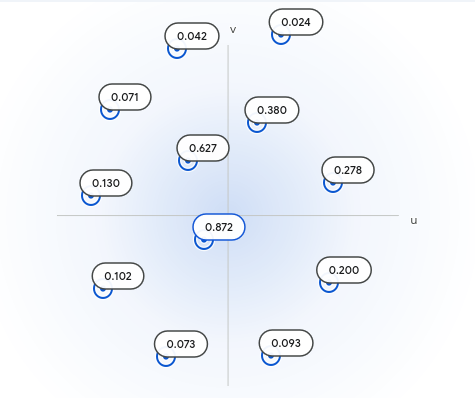
\includegraphics[width=0.8\columnwidth]{uvPlaneWeight.png}
    \caption{Two-dimensional Gaussian weighting matrix utilised as a continuous mathematical mask to prioritise the central region of the spatial frequency domain.}
    \label{fig:uv_weight}
\end{figure}

\subsection{Simulated Annealing Baseline}
Simulated annealing served as the trajectory-based baseline for the experiment. The algorithm was initialised with a 
random 16-antenna configuration and a high starting temperature. During each iteration, a neighbour solution was generated 
by swapping a single active antenna with a randomly selected inactive pad. The algorithm employed a geometric cooling 
schedule to systematically reduce the temperature. The temperature reduction transitioned the search from global 
exploration to local exploitation. The maximum fitness score achieved by the simulated annealing executions established 
the primary benchmark for evaluating the population-based approaches.

\subsection{Genetic Algorithm Variants}
To investigate the ruggedness of the MeerKAT fitness landscape, four distinct configurations of the genetic algorithm 
were constructed. All configurations utilised a static population size and an elitism mechanism. The elitism mechanism 
preserved the highest-scoring individual across generations. Furthermore, all configurations utilised an intersection 
crossover operator. The intersection crossover operator ensured the structural constraint of exactly 16 active antennas 
was strictly maintained.

The empirical process evaluated the following four evolutionary configurations:
\begin{enumerate}
    \item \textbf{Standard Baseline:} The baseline configuration utilised standard operational parameters. The parameters included a moderate tournament size and a standard mutation rate. The baseline configuration established an evolutionary performance benchmark.
    \item \textbf{Reduced Selection Pressure:} The tournament size was significantly reduced. The reduction was designed to decrease selection pressure. Decreased selection pressure allowed mathematically weaker individuals to survive longer. The survival of weaker individuals prevented the rapid domination of early local optima.
    \item \textbf{Enhanced Diversity Maintenance:} A fitness sharing mechanism utilising an expanded niche radius was implemented. The expanded radius aggressively penalised candidate configurations possessing high spatial similarity. The spatial penalty forced the population to distribute across multiple distinct peaks in the search landscape rather than converging on a single topography.
    \item \textbf{High-Frequency Mutation:} The probability of mutation was substantially increased. The increased mutation rate injected a high degree of stochastic variation into the offspring generation. The stochastic variation tested the ability of the algorithm to escape deep local optima through continuous, aggressive perturbation.
\end{enumerate}

\subsection{Fitness Sharing Mechanism}
To maintain population diversity, a fitness sharing penalty was applied to the raw fitness 
scores prior to selection. For each individual $i$, the shared fitness $f'_i$ is computed 
by dividing the raw fitness $f_i$ by the niche count $m_i$, defined as the sum of sharing 
function values across all population members:
\begin{equation}
f'_i = \frac{f_i}{m_i}, \quad \text{where} \quad m_i = \sum_{j=1}^{N} sh(d_{ij})
\end{equation}
The sharing function $sh(d_{ij})$ penalises individuals based on their Hamming distance 
$d_{ij}$, defined as the number of antenna positions that differ between two binary 
configurations. The penalty is applied within a niche radius $\sigma_{share}$:
\begin{equation}
sh(d_{ij}) = \begin{cases} 1 - \dfrac{d_{ij}}{\sigma_{share}} & \text{if } d_{ij} < \sigma_{share} \\ 0 & \text{otherwise} \end{cases}
\end{equation}
Individuals within the niche radius receive reduced effective fitness, discouraging the 
population from clustering around a single dominant solution.

To summarise, the methodology section defined the weighted $uv$-coverage density objective function. The 
section detailed the simulated annealing baseline and the four genetic algorithm configurations implemented 
to solve the discrete subset selection problem.
\section{Empirical Procedure}
\label{sec:empirical}

The empirical procedure section details the experimental setup utilised to evaluate the metaheuristic algorithms. The section begins by defining the specific experimental hypotheses and the benchmark problem. The narrative subsequently specifies the control parameters implemented for the simulated annealing baseline and the genetic algorithm variants, including explicit mathematical motivations for their selection. Finally, the section formalises the statistical testing methodology utilised to validate the research results.

\subsection{Experimental Objectives and Benchmark Problem}
The empirical study investigated the relative performance of population-based and trajectory-based metaheuristics applied to a highly deceptive search landscape. The benchmark problem utilised for evaluation was the MeerKAT 64-antenna array discrete subset selection problem. The physical coordinates of the 64 MeerKAT pads served as the static dataset.

The primary hypothesis postulated that the genetic algorithm variant utilising enhanced diversity maintenance (Variant Two) would achieve superior $uv$-coverage density compared to the standard evolutionary configurations and the simulated annealing baseline. The rugged nature of the spatial frequency landscape heavily penalises premature convergence. Therefore, explicit mathematical mechanisms designed to force population distribution across multiple local optima should theoretically yield superior global solutions. 

\subsection{Execution Environment and Sampling}
The simulated annealing algorithm and the genetic algorithm variants possess inherently stochastic properties. A single execution does not provide a reliable metric of algorithmic efficacy. Therefore, a total of 30 independent executions were performed for each distinct algorithmic configuration. The 30 independent runs ensured a statistically significant sample size for subsequent non-parametric performance analysis. A sample of 30 satisfies the conventional minimum threshold for applying the Central Limit Theorem to sample statistics and provides sufficient statistical power for the Mann-Whitney U test to detect moderate effect sizes at a significance level of $\alpha = 0.05$. No random seeds were fixed across executions; all stochastic initialisations drew independently from the system entropy pool to guarantee genuine run independence.

All algorithms were implemented utilising the Python programming language. The executions were conducted on a Fedora Linux operating system environment. To ensure a standardised comparison, all independent executions utilised the identical weighted $uv$-coverage objective function detailed in Section 3.1. 

\subsection{Simulated Annealing Configuration}
The simulated annealing algorithm required the specification of an initial temperature, an iteration limit, and a cooling schedule multiplier. The initial temperature was set to 1000. An initial temperature of 1000 was selected by evaluating the Metropolis acceptance probability $P = e^{\Delta f / T}$ at the expected scale of fitness differences in the search space. At $T = 1000$, a candidate solution 200 fitness points inferior to the current solution retains an acceptance probability of $e^{-200/1000} \approx 0.82$, ensuring that the algorithm explores the landscape broadly during the initial phase rather than committing prematurely to a local optimum. A geometric cooling multiplier of 0.99999 was applied at the conclusion of each iteration. The 0.99999 multiplier was selected specifically to force an extremely slow, gradual thermodynamic transition from global exploration to localised exploitation over hundreds of thousands of iterations. 

To guarantee equitable computational expenditure across the differing heuristic methodologies, the simulated annealing algorithm executed for exactly 500,000 iterations. The iteration limit perfectly matched the total number of objective function evaluations performed by the genetic algorithms.

\subsection{Genetic Algorithm Configurations}
The four genetic algorithm configurations shared a common foundational structure. All variants utilised a static population size of 500 individuals. The evolutionary process executed for a maximum of 1000 generations per independent run. The multiplication of 500 individuals by 1000 generations yielded a maximum of 500,000 objective function evaluations per execution. An intersection crossover operator was applied unconditionally during parent recombination. Furthermore, a strict elitism mechanism preserved the single highest-scoring individual across every generation boundary.

The experimental variants modified specific control parameters to isolate the effects of selection pressure, diversity maintenance, and mutation frequency. The exact parameter configurations for the four evolutionary variants are summarised in Table~\ref{tab:ga_parameters}. 

\begin{table}[htbp]
    \centering
    \caption{Control parameters applied to the genetic algorithm variants during the empirical evaluation.}
    \label{tab:ga_parameters}
    \setlength{\tabcolsep}{4pt}
    \renewcommand{\arraystretch}{1.05}
    \footnotesize
    \resizebox{\columnwidth}{!}{%  <--- CHANGED THIS LINE
        \begin{tabular}{@{}lccc@{}}
            \toprule
            \textbf{Configuration} & \textbf{Tournament Size} & \textbf{Mutation Rate} & \textbf{Niche Radius} \\
            \midrule
            Standard Baseline & 5 & 0.15 & N/A \\
            Variant One Reduced Selection & 2 & 0.15 & N/A \\
            Variant Two Enhanced Diversity & 5 & 0.15 & 12 \\
            Variant Three High Mutation & 3 & 0.25 & N/A \\
            \bottomrule
        \end{tabular}%
    }
\end{table}

The Standard Baseline utilised a tournament size of five and a mutation probability of 0.15. A tournament size of five provided strong, 
baseline selection pressure. Tournament selection exerts pressure proportional to tournament size: a larger pool increases the probability that the highest-fitness individual is selected, thereby amplifying the reproductive advantage of superior configurations. A size of five was selected to provide directed exploitation without eliminating the stochastic variation required for continued exploration. Variant One reduced the tournament size to two. The reduction to two minimised selection pressure, 
thereby allowing mathematically weaker individuals to survive longer and preventing the rapid domination of early local optima. 
Variant Two implemented an expanded fitness sharing penalty utilising a niche radius of 12. A radius of 12 aggressively penalised 
structurally similar antenna layouts to enforce the primary hypothesis. Variant Three substantially increased the mutation probability 
to 0.25 to test the ability of the algorithm to escape deep local optima through continuous, high-frequency stochastic perturbation.

\subsection{Statistical Analysis Methodology}
The final fitness scores generated by the 30 independent executions were aggregated for statistical comparison. Metaheuristic search 
trajectories rarely produce normally distributed performance data. Consequently, parametric statistical tests that assume a Gaussian distribution are invalid. 

The two-tailed Mann-Whitney U test was selected to evaluate the statistical significance of the performance differences between 
the algorithms. The Mann-Whitney U test is a robust, non-parametric method used to determine whether two independent samples 
were drawn from populations with the same distribution. The null hypothesis for each pairwise comparison was defined as $H_0$: the two independent samples of final fitness scores were drawn from populations with identical distributions, implying no significant performance difference between the two algorithmic configurations. The alternative hypothesis $H_1$ postulated that a significant distributional difference existed. A significance level of $\alpha = 0.05$ was established for all statistical 
comparisons. A calculated $p$-value less than 0.05 successfully rejects the null hypothesis and confirms that the difference in algorithmic 
performance is statistically significant.

To summarise, the empirical procedure section formalised the benchmark array subset problem and the diversity maintenance hypothesis. 
The section detailed the computational budgets, control parameter motivations, and non-parametric statistical methodologies utilised 
to ensure rigorous, reproducible experimentation.

\section{Research Results}
 
The research results section presents the empirical data collected during the 30 independent
executions of the implemented metaheuristics. The section begins by detailing the summary
statistics to evaluate overall algorithmic robustness. Subsequently, the convergence profiles
are analysed to assess exploration and exploitation behaviours, including an examination of
whether the observed outcomes were expected and how alternative experimental conditions would
alter them. The section then reports the results of the non-parametric statistical tests to
validate the performance differences and evaluate the initial hypothesis. Finally, the optimal
configuration topographies are analysed to provide a geometric explanation for the advantage of the dominant
algorithm.
 
% ------------------------------------------------------------
\subsection{Summary Statistics}
% ------------------------------------------------------------
 
Table~\ref{tab:summary_stats} presents the aggregated performance metrics across the 30
independent executions for each algorithmic configuration, ranked in descending order of mean
performance. The primary metric for evaluation was the final weighted $uv$-coverage density
score achieved at the termination of the computational budget.
 
\begin{table}[htbp]
    \centering
    \caption{Summary statistics of the final objective function scores across 30 independent
             executions, ranked by mean performance.}
    \label{tab:summary_stats}
    \setlength{\tabcolsep}{4pt}
    \renewcommand{\arraystretch}{1.1}
    \footnotesize
    \resizebox{\columnwidth}{!}{%
        \begin{tabular}{@{}lcccc@{}}
            \toprule
            \textbf{Algorithm} & \textbf{Max} & \textbf{Min} & \textbf{Mean} & \textbf{Std.\ Dev.} \\
            \midrule
            Simulated Annealing         & 14938.94 & 14816.51 & 14926.24 & 26.70 \\
            GA: Standard Baseline       & 14781.16 & 14621.76 & 14683.01 & 37.87 \\
            GA: Variant Two (Diversity) & 14695.71 & 14571.06 & 14615.30 & 35.84 \\
            GA: Variant Three (Mutation)& 14571.19 & 14373.44 & 14452.49 & 48.64 \\
            GA: Variant One (Selection) & 14531.06 & 14374.84 & 14449.83 & 44.15 \\
            \bottomrule
        \end{tabular}%
    }
\end{table}
 
Simulated annealing achieved the highest maximum fitness score of 14938.94, the highest mean
score of 14926.24, and the narrowest performance range of 122.43 points across all 30 runs.
The low standard deviation of 26.70 and the narrow range together confirm that the
trajectory-based configuration was highly robust, consistently discovering near-optimal regions
of the search landscape regardless of stochastic initialisation. The outcome is consistent
with the theoretical expectation that a slow geometric cooling schedule would allow the
algorithm to converge reliably from any starting point, as the Metropolis criterion suppresses
the influence of the initial random configuration during the high-temperature exploration phase.
 
Conversely, all four genetic algorithm configurations failed to surpass the simulated annealing
baseline. The Standard Baseline achieved the highest mean among evolutionary configurations at
14683.01, representing a deficit of 243.23 points relative to the simulated annealing mean.
Variant One and Variant Three exhibited the highest standard deviations of 44.15 and 48.64
respectively, and the widest performance ranges, indicating severe run-to-run inconsistency.
The elevated variance in these configurations suggests that reducing selection pressure or
increasing the mutation rate made the algorithms highly sensitive to the stochastic conditions
of each individual run, producing outcomes that were difficult to predict or replicate.
 
% ------------------------------------------------------------
\subsection{Convergence Analysis}
% ------------------------------------------------------------
 
Figure~\ref{fig:convergence_full} illustrates the macroscopic average convergence profiles of
all algorithms across the full 500,000-evaluation budget. Figure~\ref{fig:convergence_zoom}
provides an isolated perspective of the upper performance range to highlight the late-stage
exploitation dynamics and final performance discrepancies between configurations.
 
\begin{figure}[htbp]
    \centering
    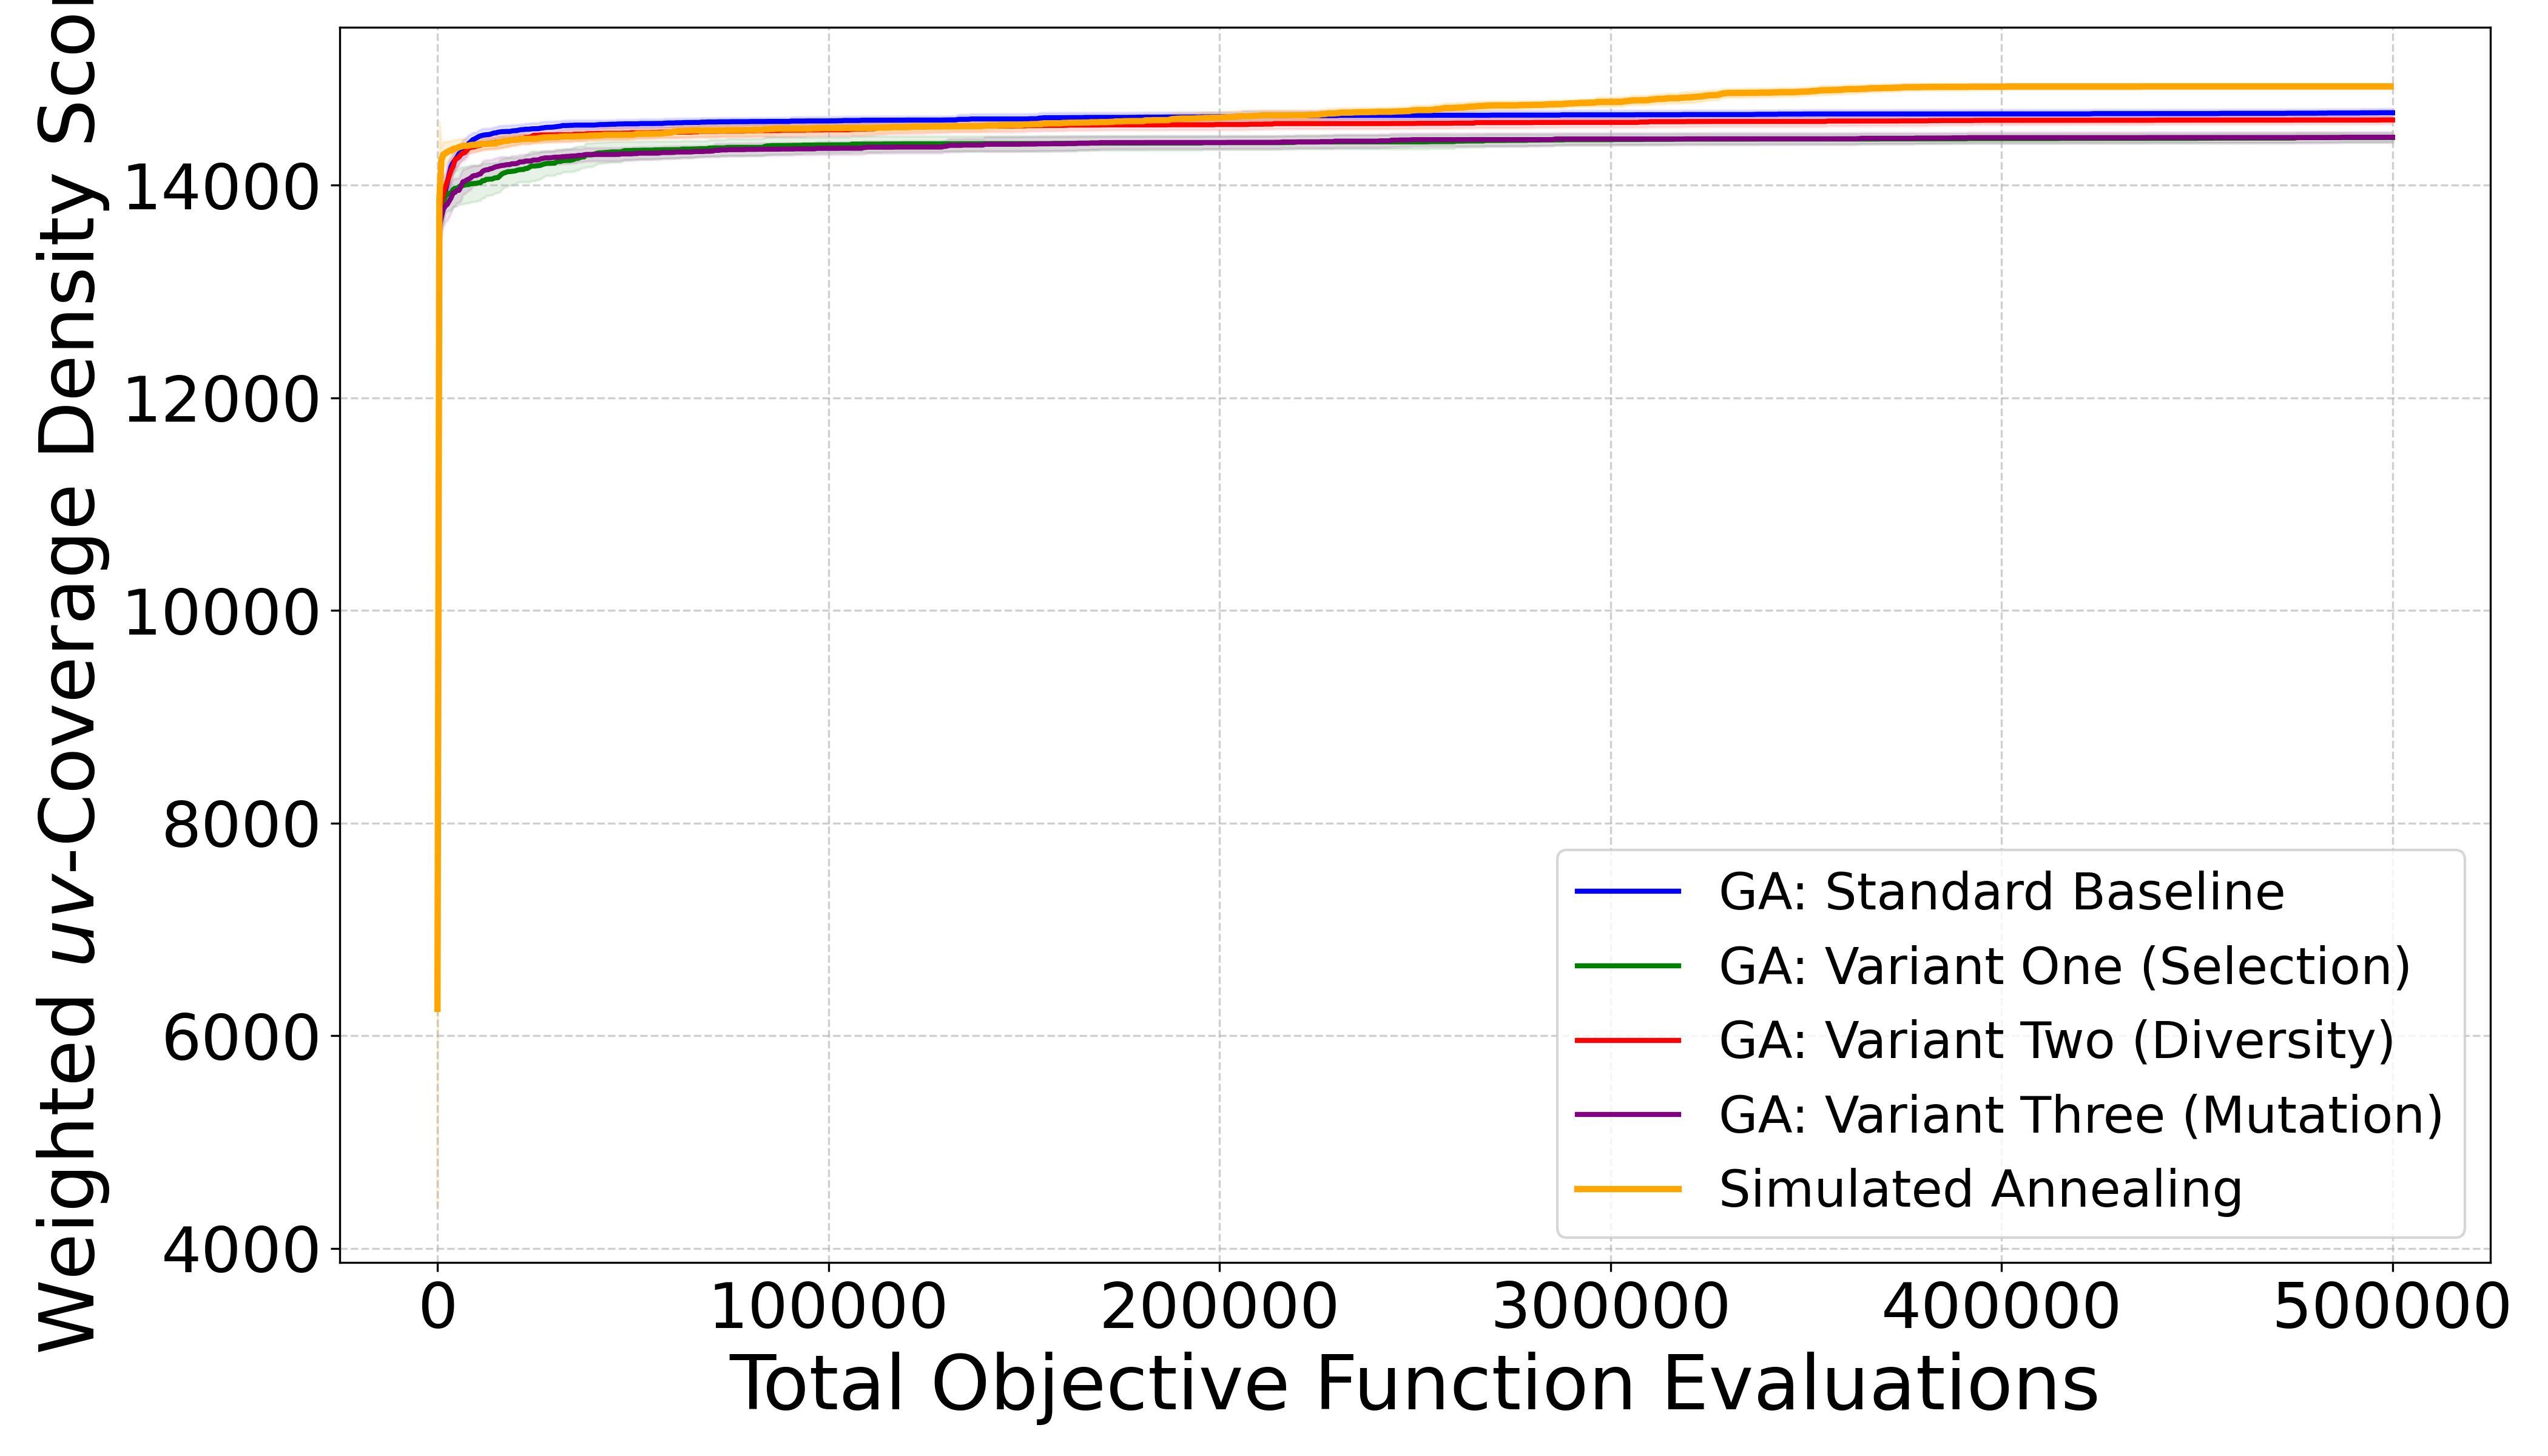
\includegraphics[width=\linewidth]{../out/convergence_comparison_30runs.png}
    \caption{Macroscopic average convergence trajectories illustrating the rapid initialisation
             and early exploration phase across all configurations.}
    \label{fig:convergence_full}
\end{figure}
 
\begin{figure}[htbp]
    \centering
    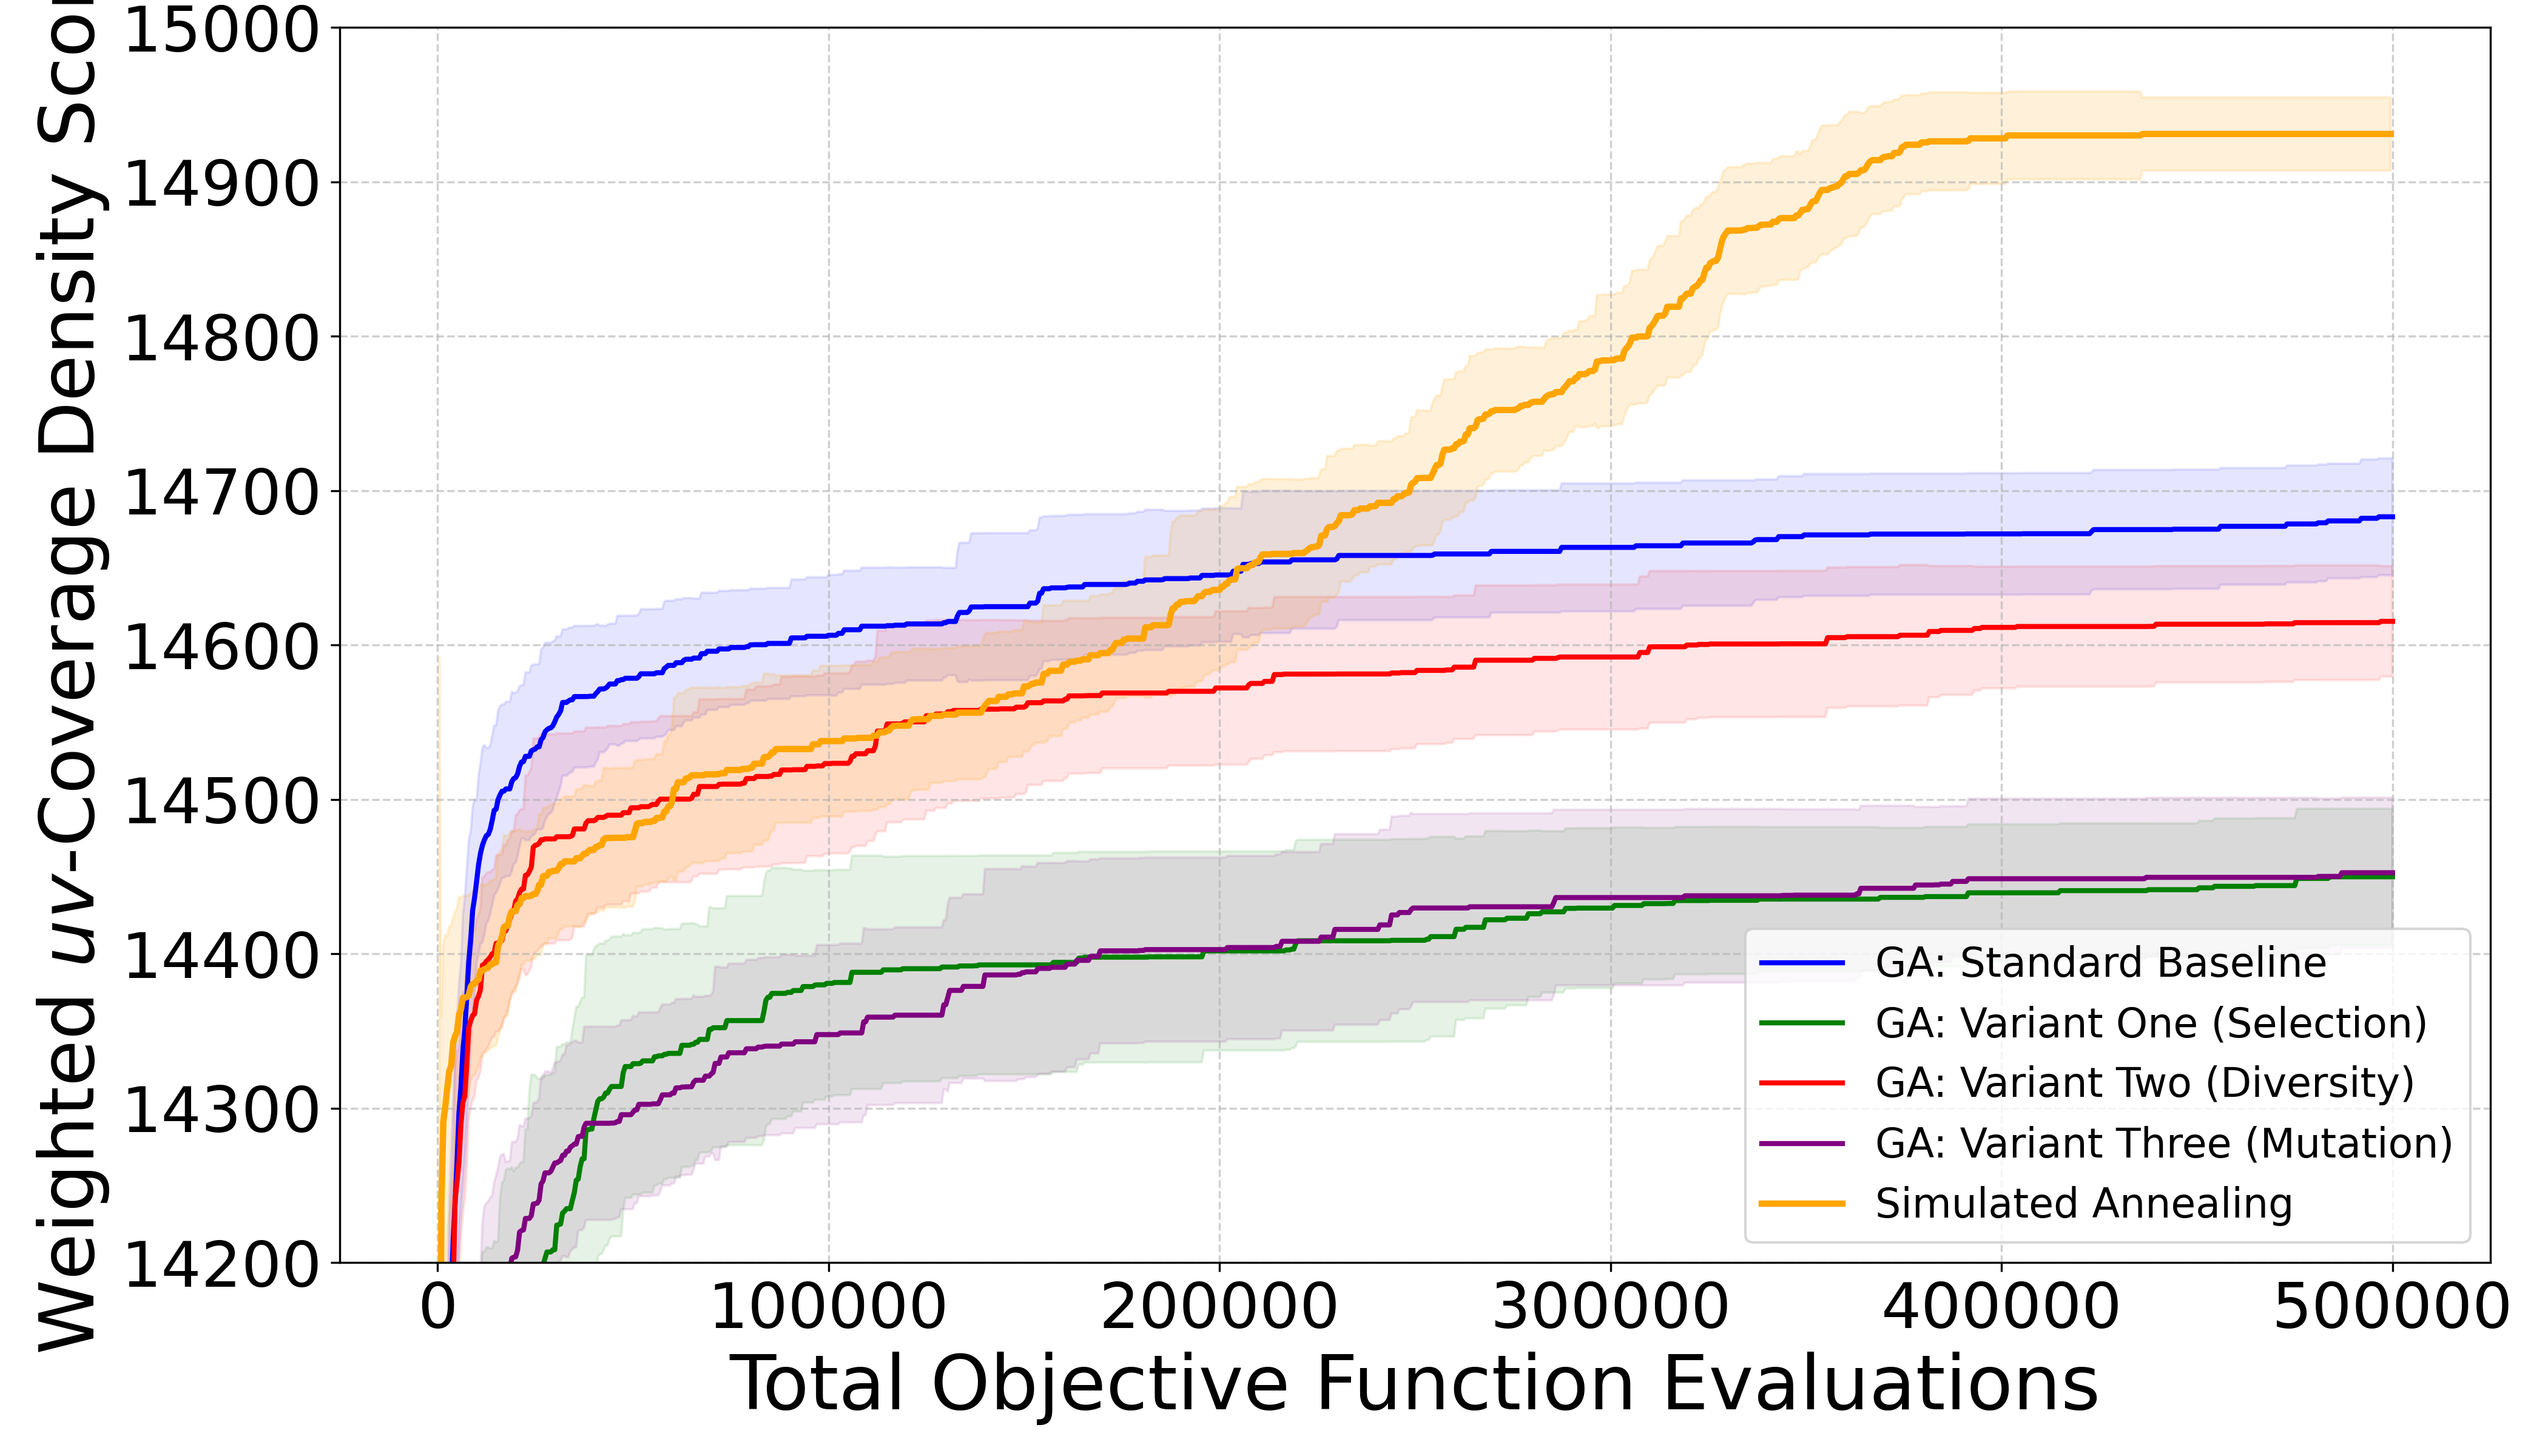
\includegraphics[width=\linewidth]{../out/zoomed_convergence_comparison_30runs.png}
    \caption{Isolated convergence trajectories illustrating the late-stage exploitation phase
             and final objective scores.}
    \label{fig:convergence_zoom}
\end{figure}
 
\subsubsection{Simulated Annealing Trajectory}
The macroscopic view confirms that simulated annealing began with the lowest initial
performance among all configurations. The expected behaviour of a trajectory-based
algorithm initialising from a single random 16-antenna layout: the first evaluation reflects
purely random placement, and the cooling schedule must invest many early iterations in
thermodynamic exploration before meaningful exploitation can occur. Despite this slow start,
the algorithm demonstrated continuous, uninterrupted improvement throughout the full evaluation
budget. By approximately 200,000 evaluations, simulated annealing surpassed the final
performance of the Standard Baseline GA and continued to improve for the remaining 300,000
iterations. The sustained late-stage gain is consistent with the theoretical behaviour of a
well-calibrated geometric cooling schedule, wherein the temperature decreases sufficiently
slowly to permit fine-grained local refinement during the final exploitation phase.
 
\subsubsection{Genetic Algorithm Convergence and Plateau}
The baseline genetic algorithm and all three of its variants exhibited a markedly different
convergence profile. All evolutionary configurations achieved rapid performance gains within
the first 50,000 evaluations, rising from random initialisation to scores in the range of
14,300--14,600. However, as evidenced in Figure~\ref{fig:convergence_zoom}, all four genetic
algorithm variants plateaued at approximately 150,000 evaluations, after which no meaningful
improvement was observed across the remaining 350,000 evaluations. The early stagnation was
not expected at the outset of the study, given that the intersection crossover operator was
specifically designed to preserve structural constraints and propagate high-performing
sub-configurations.
 
The premature convergence is most plausibly attributed to the destructive nature of the
intersection crossover operator in this specific discrete landscape. When two high-performing
16-antenna layouts share only a small subset of common active pads, the crossover operation
randomly distributes the remaining positions. The random distribution destroys the specific
geometric neighbourhood relationships between antenna pairs that produce high-density UV tracks.
The recombination therefore creates offspring that are structurally novel but perform no better
than their parents. The shaded standard deviation bands in both figures provide additional
evidence: the relatively wide bands around all GA configurations, particularly visible in
Figure~\ref{fig:convergence_zoom}, confirm high run-to-run variability that is characteristic
of a population prematurely trapped in a local optimum basin.
 
\subsubsection{Analysis of Individual Variant Behaviours}
The three GA variants exhibited distinct failure modes that illuminate the landscape topology
of the MeerKAT subset selection problem.
 
Variant One reduced the tournament size from five to two, which minimised selection pressure
and introduced a degree of genetic drift into the population dynamics. With weak selection
pressure, the algorithm failed to consistently amplify high-fitness antenna pairings across
generations. The population effectively performed a near-random walk across the configuration
space rather than a directed search. The consequence was the lowest mean performance among all
configurations at 14449.83, confirming that an absence of selection pressure is as harmful as
premature convergence on this rugged landscape.
 
Variant Three increased the mutation rate from 0.15 to 0.25. In this discrete binary domain,
mutation operates by swapping an active antenna with an inactive pad. At a rate of 0.25, each
individual active antenna position has a 25\% probability of being displaced per generation.
For a 16-antenna configuration, this implies that on average four antenna positions are
perturbed in every offspring, constituting a structural change of 25\% of the entire active
array. While high mutation theoretically enables escape from local optima, the perturbation
magnitude was too large to permit fine-grained exploitation of high-fitness regions. Well-adapted
antenna sub-groupings were disrupted by mutation at a rate faster than selection could rebuild
them, resulting in a mean performance of 14452.49 that was marginally superior to Variant One
but still substantially below the Standard Baseline.
 
Variant Two, which implemented an expanded fitness sharing niche radius of 12, exhibited
convergence trajectories that were consistently below the Standard Baseline despite utilising
identical selection pressure and mutation parameters. The expanded radius aggressively penalised
structurally similar individuals, forcing the population to distribute across multiple distinct
fitness peaks. However, the penalty function effectively reduced the selective advantage of the
highest-performing configurations by equalising their adjusted fitness with that of inferior
alternatives. As a result, the algorithm retained mathematically inferior candidate solutions
in the population in exchange for diversity that provided no benefit, given that the
near-optimal configurations were clustered in a single well-defined region of the search space.
 
\subsubsection{Sensitivity to Experimental Conditions}
The observed performance hierarchy is contingent on the specific topology of the objective
function. The Gaussian weighting matrix heavily prioritises central $uv$-plane density, which
intrinsically rewards configurations with dense short-baseline geometries. A flat, uniform
weighting scheme would assign equal value to all sampled $uv$-plane pixels regardless of
position. Under such a scheme, configurations maximising the raw spatial coverage footprint
would be favoured, potentially reversing the performance relationship between the centrally
clustered SA solution and the more dispersed GA configurations. Similarly, the GA stagnation
observed at 150,000 evaluations was not a consequence of an insufficient budget. The
convergence plots confirm that the evolutionary trajectories had fully flattened before this
threshold, and extending the generational limit beyond 1,000 generations would not recover
performance lost to the destructive crossover mechanism. Fundamental algorithmic changes, such
as adopting a uniform crossover operator that does not rely on shared antenna positions or
implementing a problem-specific repair operator, would be required to overcome the stagnation.
Conversely, a more aggressive SA cooling multiplier, such as 0.9999 rather than the employed
0.99999, would reduce the number of iterations available for fine-grained local exploitation
and would likely narrow the performance gap between simulated annealing and the best GA
configuration.
 
% ------------------------------------------------------------
\subsection{Statistical Significance}
% ------------------------------------------------------------
 
The summary statistics indicated a substantial performance discrepancy between the algorithms.
To determine whether the observed differences were statistically significant, two-tailed
Mann-Whitney U tests were executed utilising a significance threshold of $\alpha = 0.05$.
The Mann-Whitney U test was selected due to its non-parametric nature, as metaheuristic
performance distributions cannot be assumed to be Gaussian.
 
Comparison of the Standard Baseline GA against simulated annealing yielded a $p$-value of
$1.88445 \times 10^{-11}$. The calculated value was strictly less than the $\alpha$ threshold by
a margin of eleven orders of magnitude. Therefore, the null hypothesis was rejected. The
statistical rejection definitively confirms that the simulated annealing algorithm was
significantly superior to the best evolutionary configuration for the discrete MeerKAT antenna
placement problem. Furthermore, the magnitude of the $p$-value indicates that this superiority
is not a marginal or borderline result but a robust and decisive outcome that would be
reproduced under any reasonable significance threshold.
 
A comparison of Variant Two against the Standard Baseline GA yielded a $p$-value of $1.00$.
A value of 1.00 indicates that the direction of the test statistic was entirely opposed to the
stated hypothesis: the performance distribution of Variant Two lay strictly below that of the
Standard Baseline in every single one of the 30 independent executions. The expanded niche
radius did not merely fail to improve performance; it actively and consistently degraded it.
Consequently, the primary experimental hypothesis formulated in the Empirical Procedure section
was completely invalidated. Aggressive diversity maintenance via fitness sharing provided no
mathematical advantage on this objective function and constituted a net harm to the
exploitation capabilities of the evolutionary search.


\subsection{Optimal Configuration Topography}

To contextualise the numerical dominance of the simulated annealing algorithm, the geometric
topographies of the absolute best configurations discovered by each metaheuristic class were
analysed. Figure~\ref{fig:ga_physical} and Figure~\ref{fig:sa_physical} illustrate the
physical spatial distributions of the highest-scoring 16-antenna layouts discovered by the
genetic algorithm and simulated annealing respectively. Figure~\ref{fig:ga_uv} and
Figure~\ref{fig:sa_uv} present the corresponding high-fidelity $uv$-coverage tracks,
generated using a high-resolution simulation of 500 time steps over an eight-hour observation
window projected onto a $1024 \times 1024$ spatial frequency grid.

\begin{figure}[htbp]
    \centering
    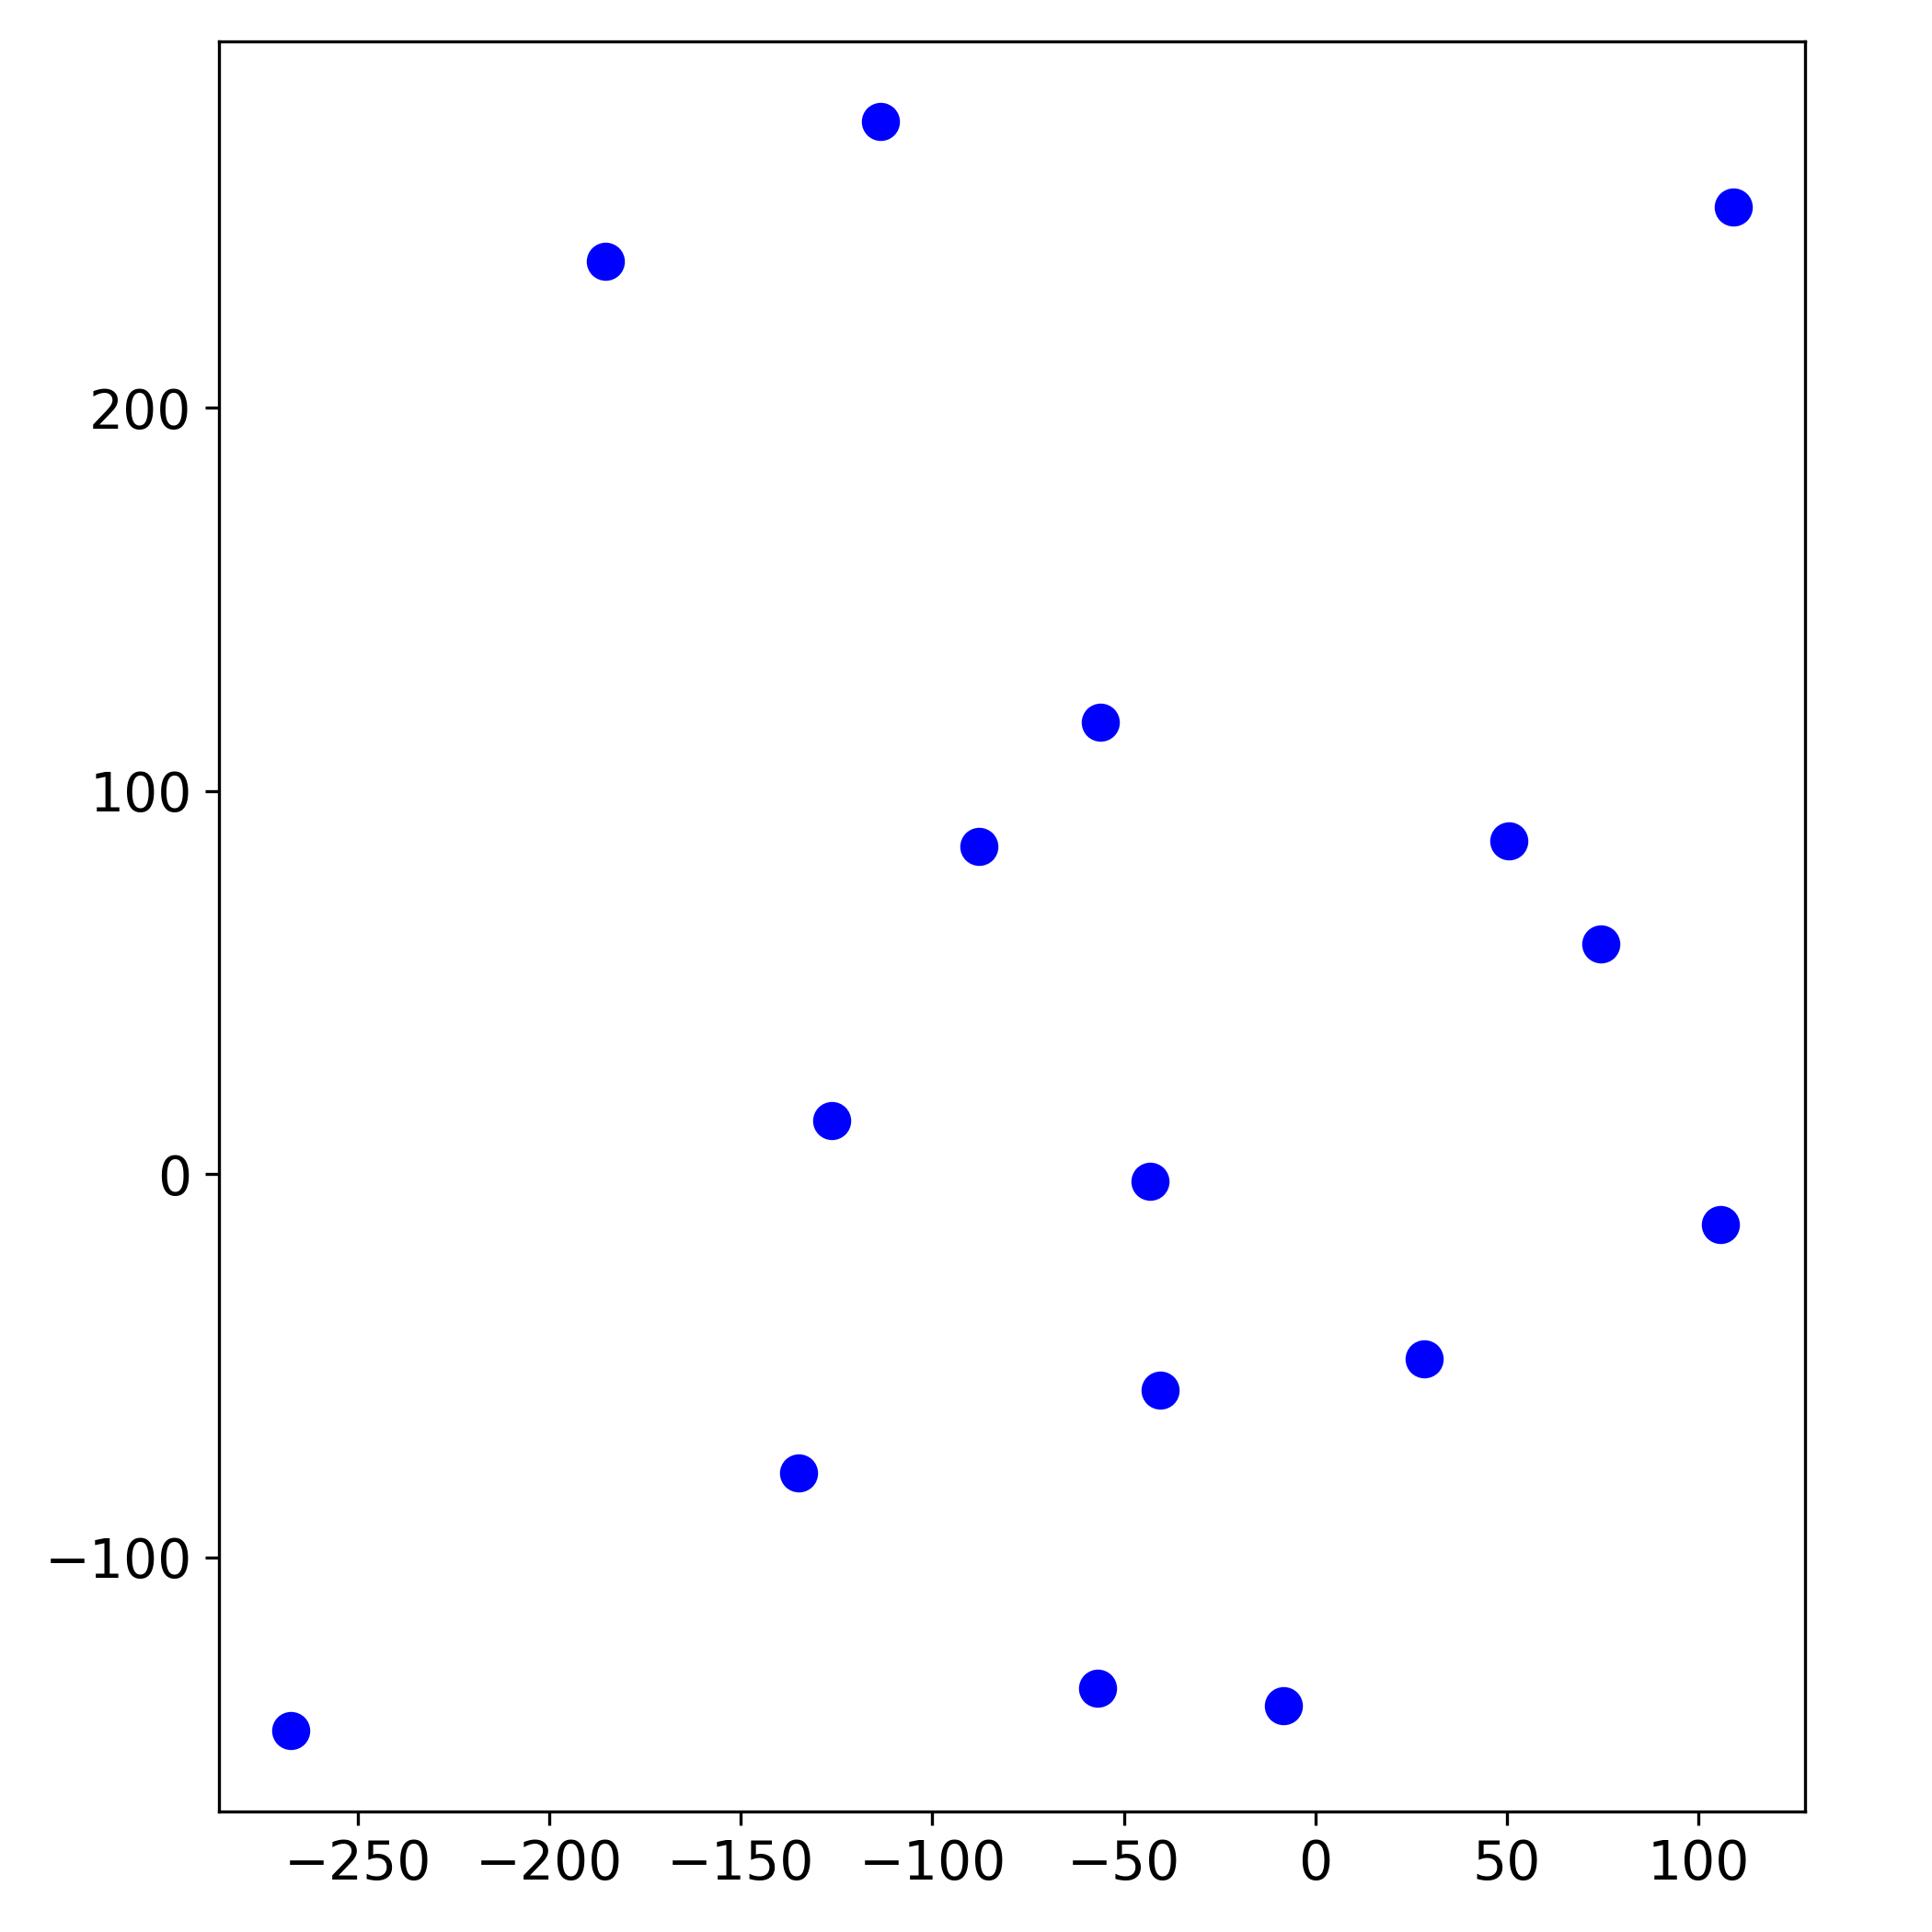
\includegraphics[width=\linewidth]{../out/ga_physical.png}
    \caption{Physical spatial layout of the optimal 16-antenna configuration discovered by
             the baseline genetic algorithm. Antenna positions are plotted in East-North-Up
             coordinates relative to the MeerKAT array reference point.}
    \label{fig:ga_physical}
\end{figure}

\begin{figure}[htbp]
    \centering
    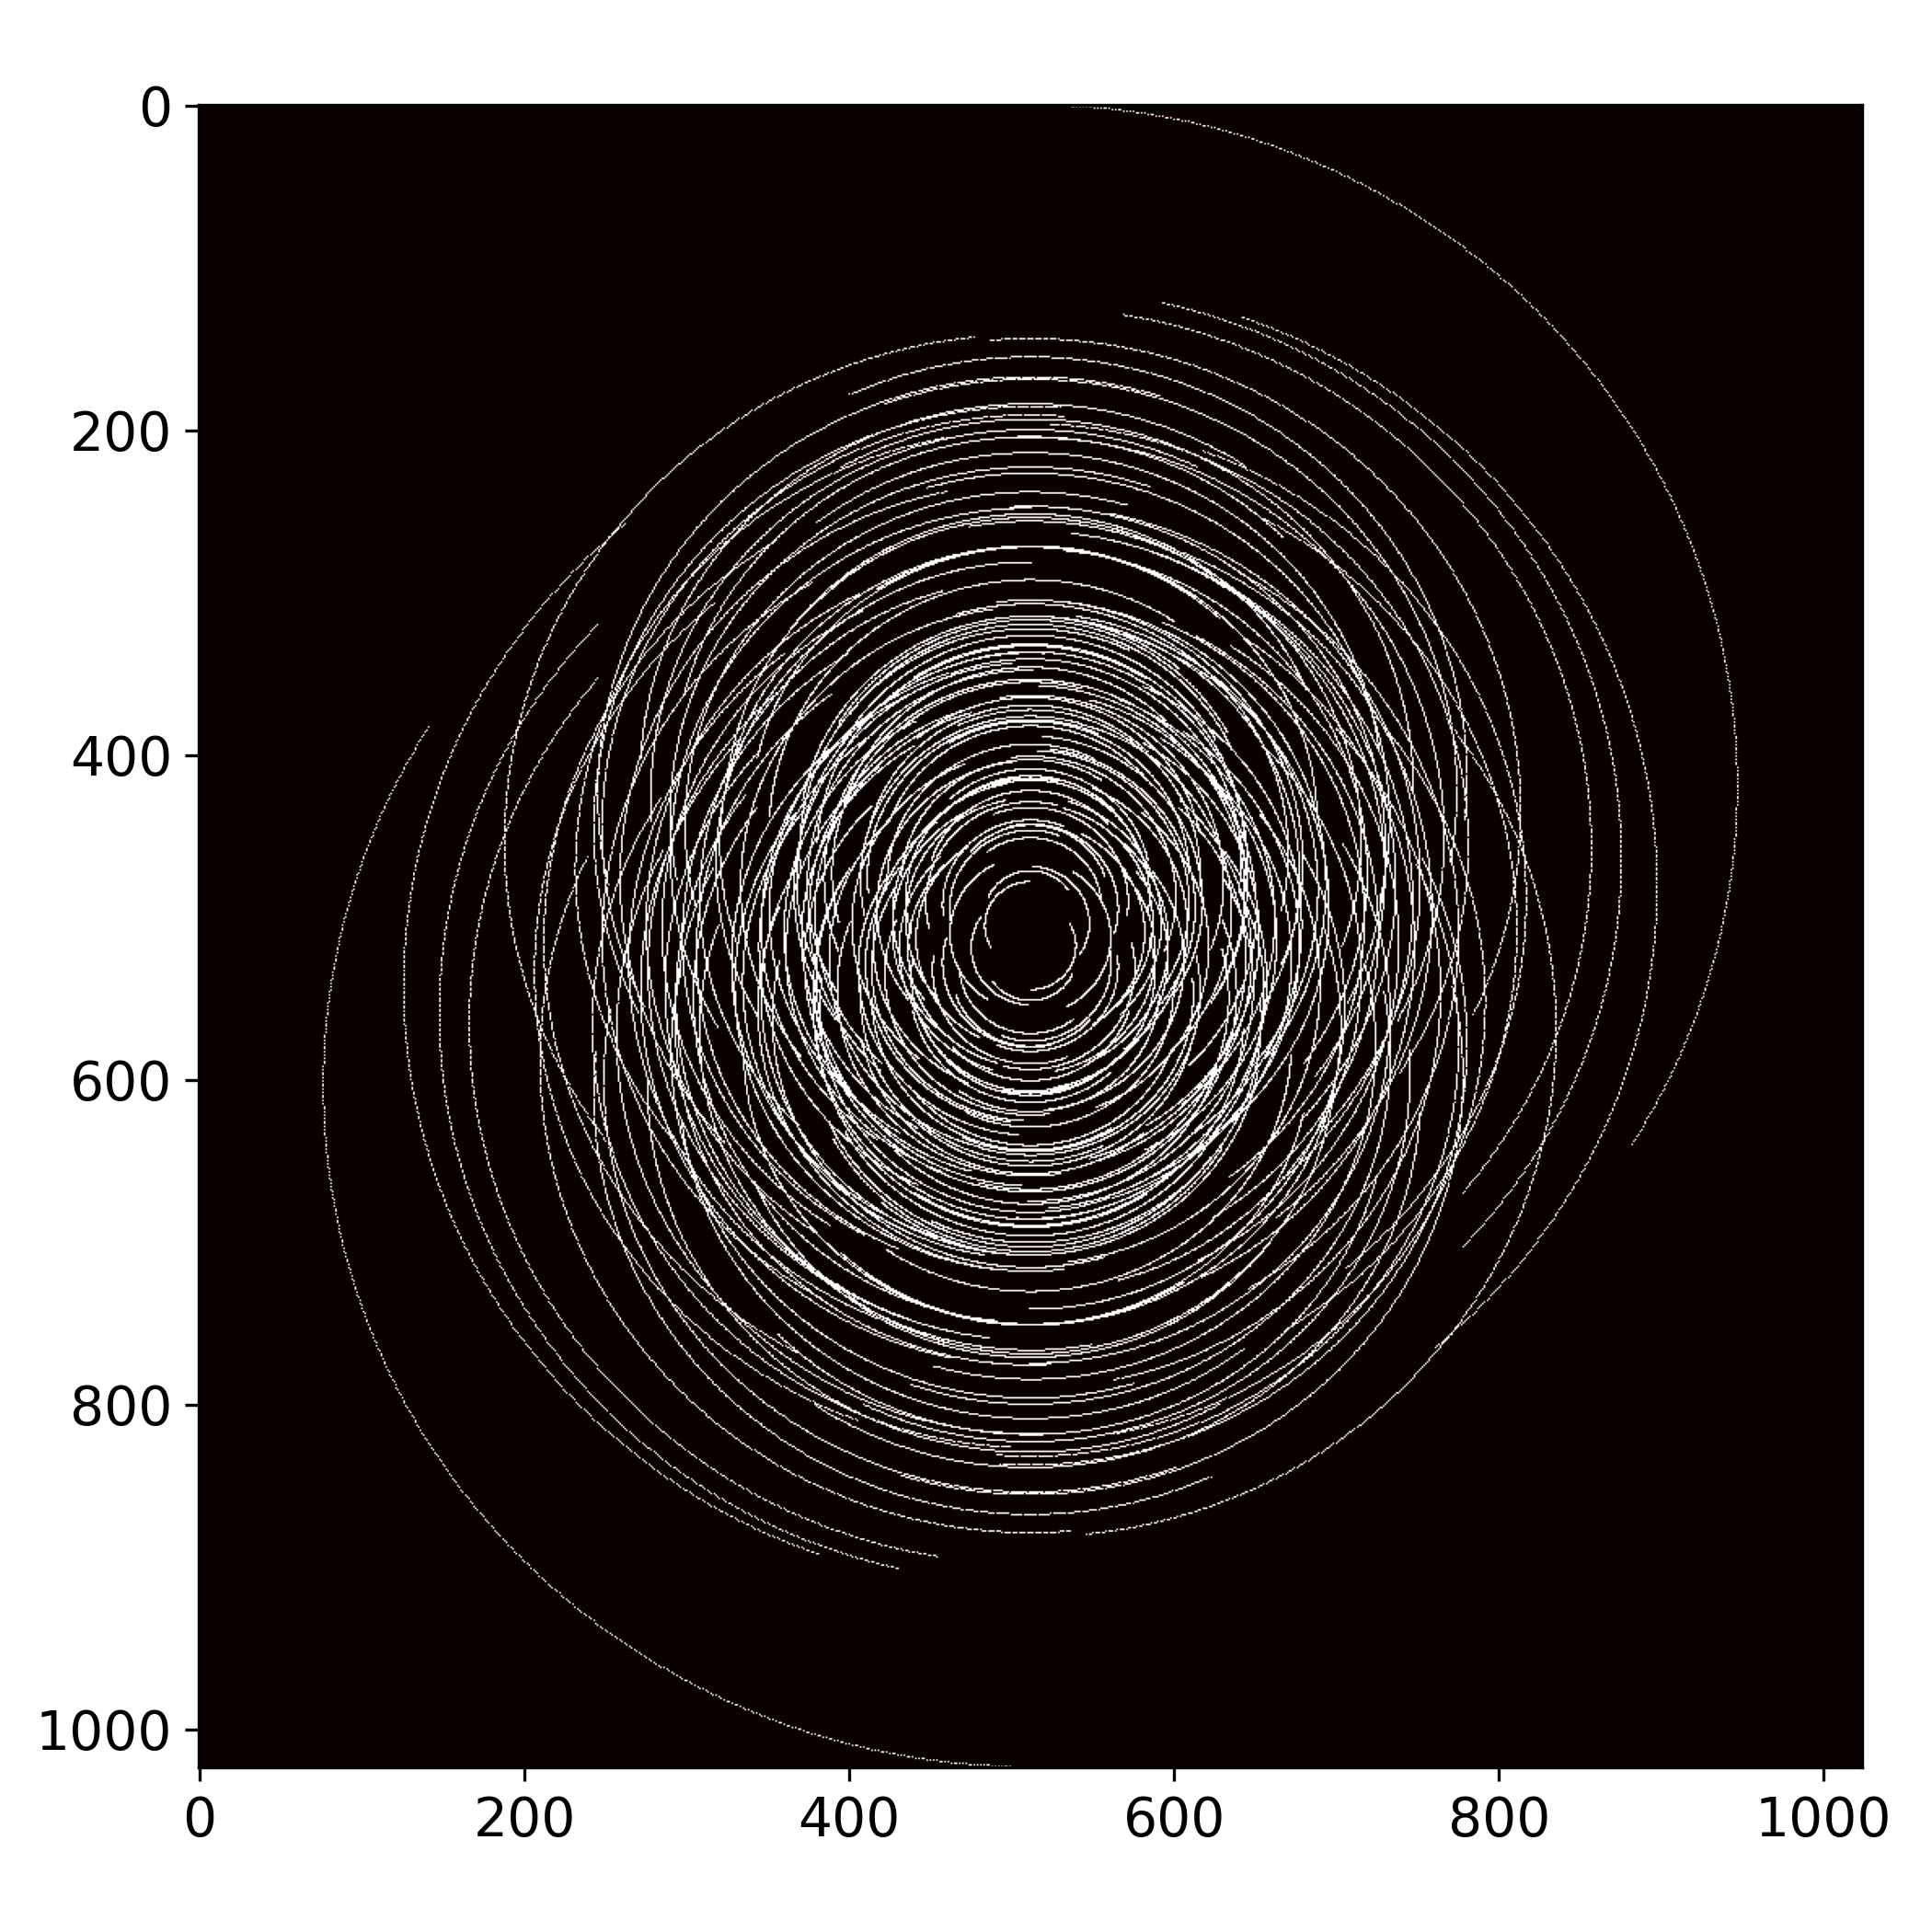
\includegraphics[width=\linewidth]{../out/ga_uv.png}
    \caption{High-resolution $uv$-coverage tracks generated by the optimal genetic algorithm
             layout.}
    \label{fig:ga_uv}
\end{figure}

\begin{figure}[htbp]
    \centering
    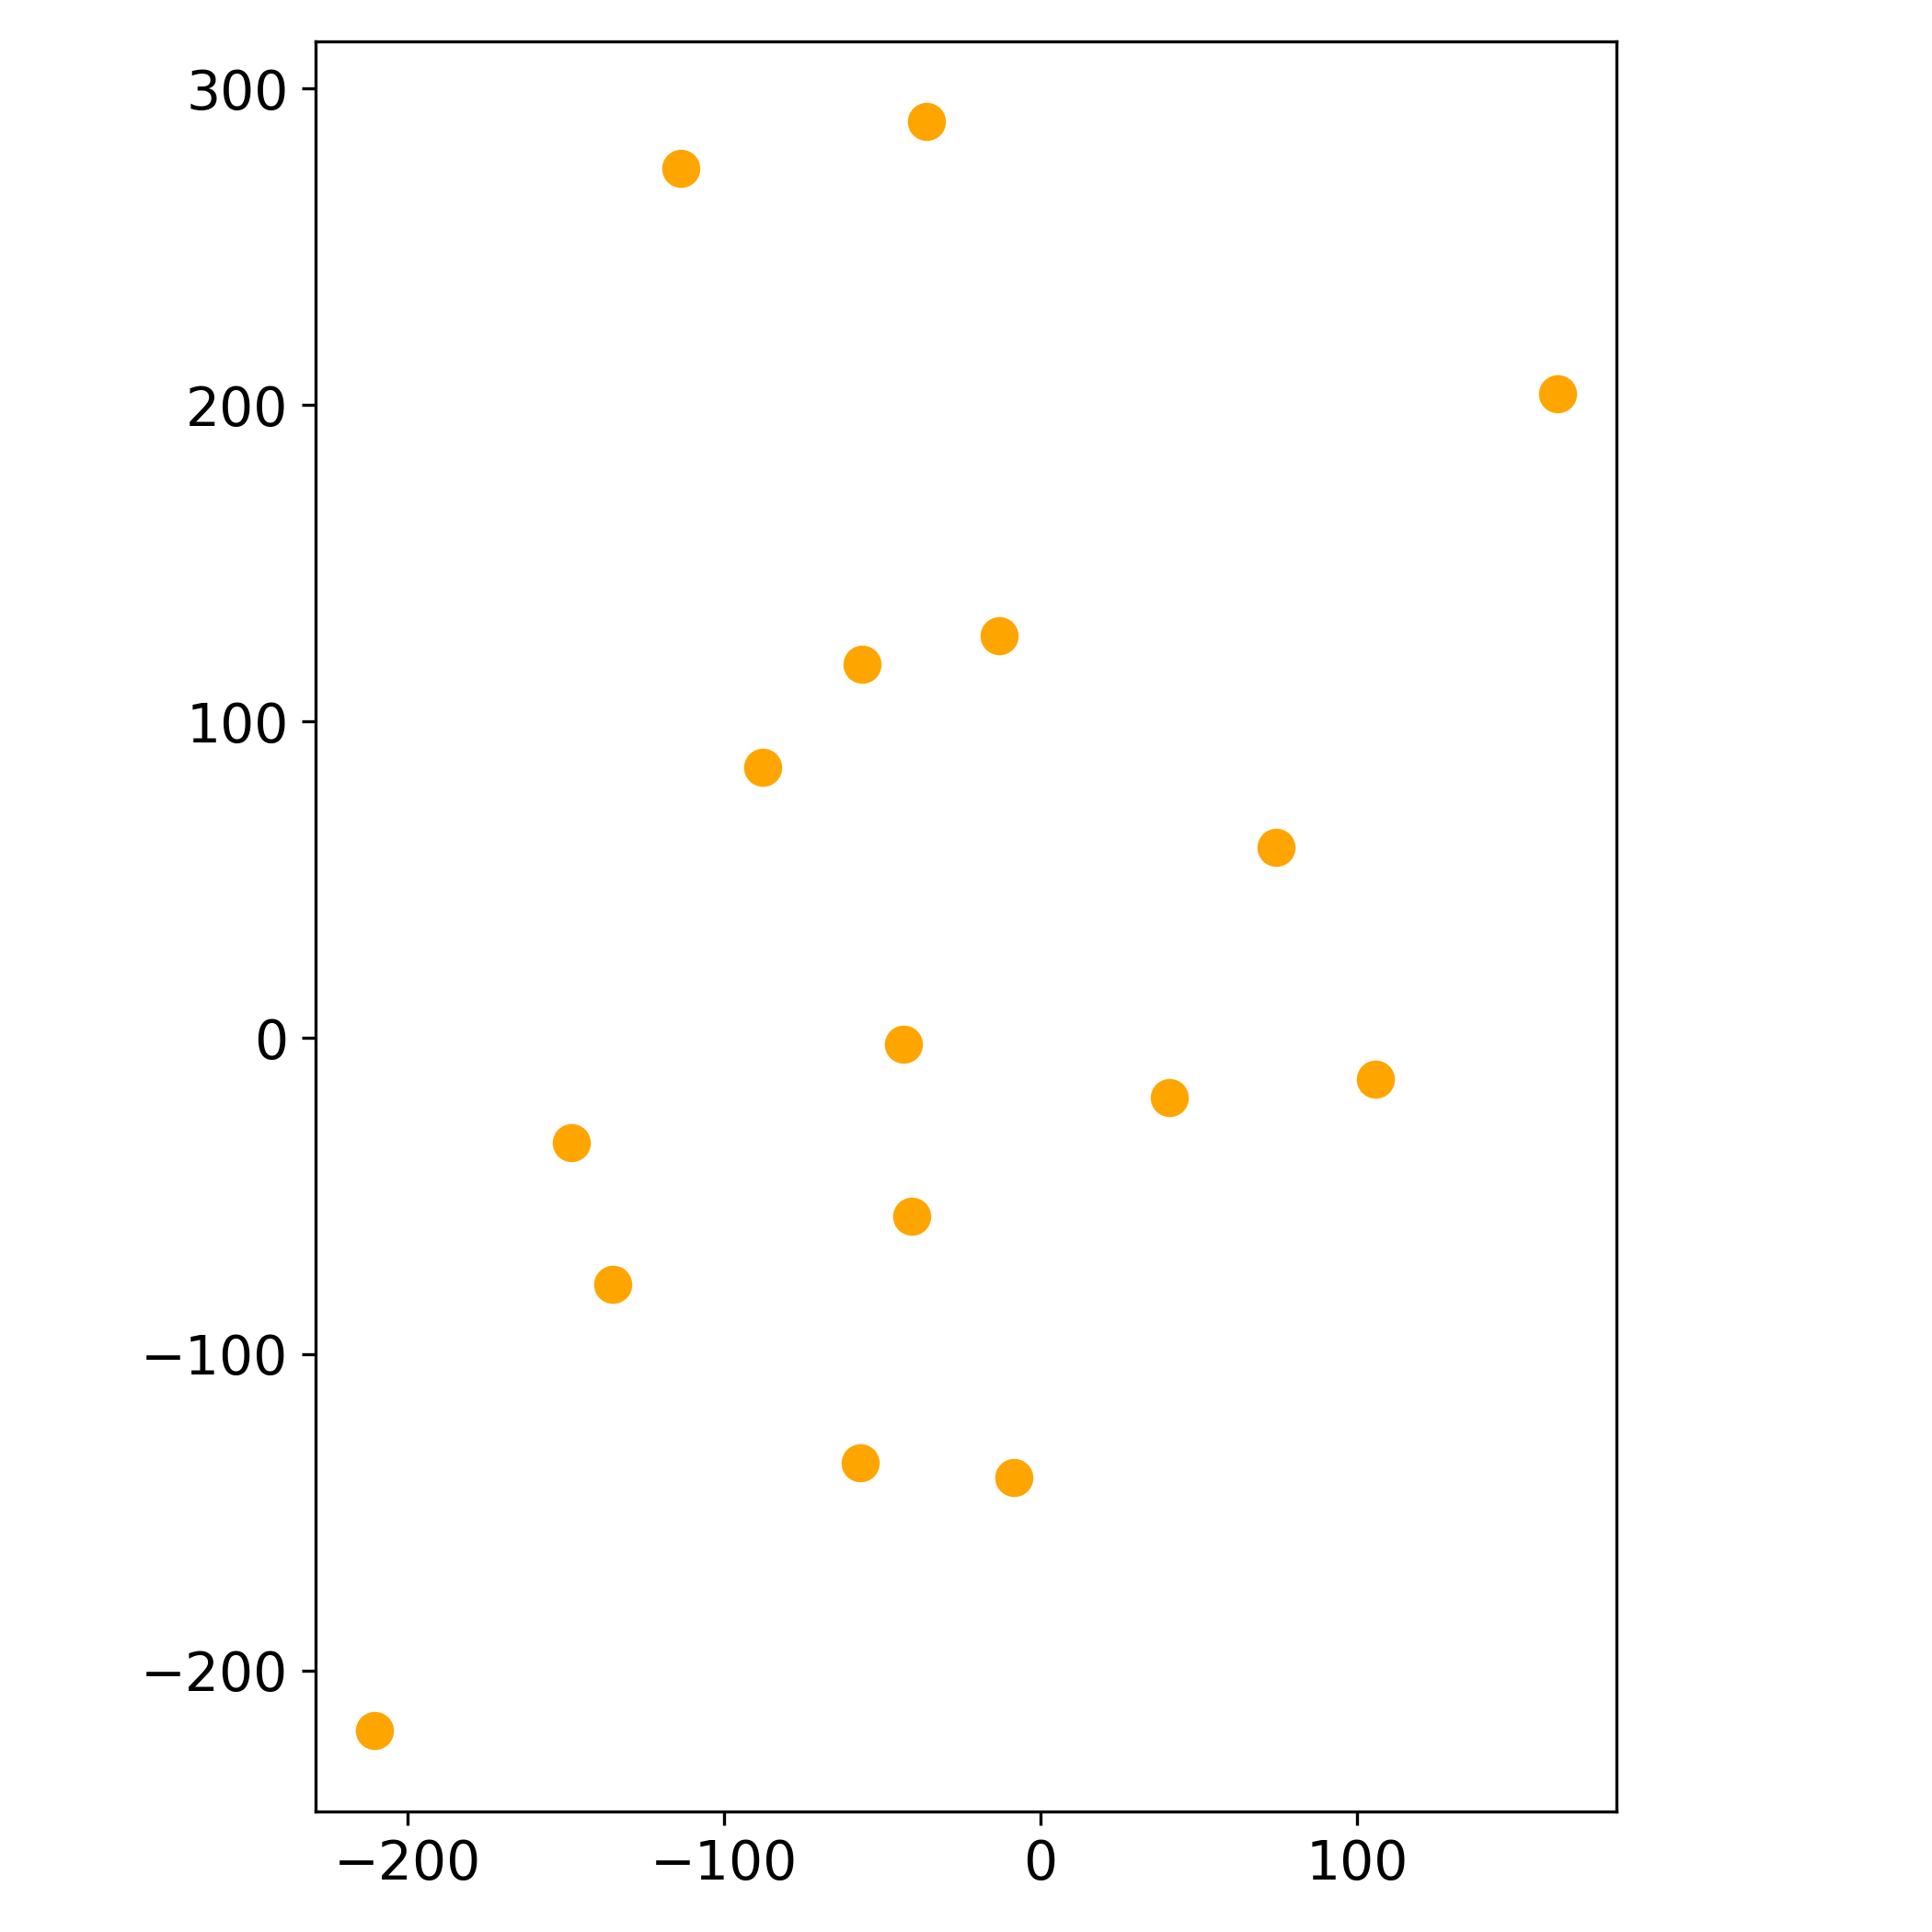
\includegraphics[width=\linewidth]{../out/sa_physical.png}
    \caption{Physical spatial layout of the optimal 16-antenna configuration discovered by
             simulated annealing.}
    \label{fig:sa_physical}
\end{figure}

\begin{figure}[htbp]
    \centering
    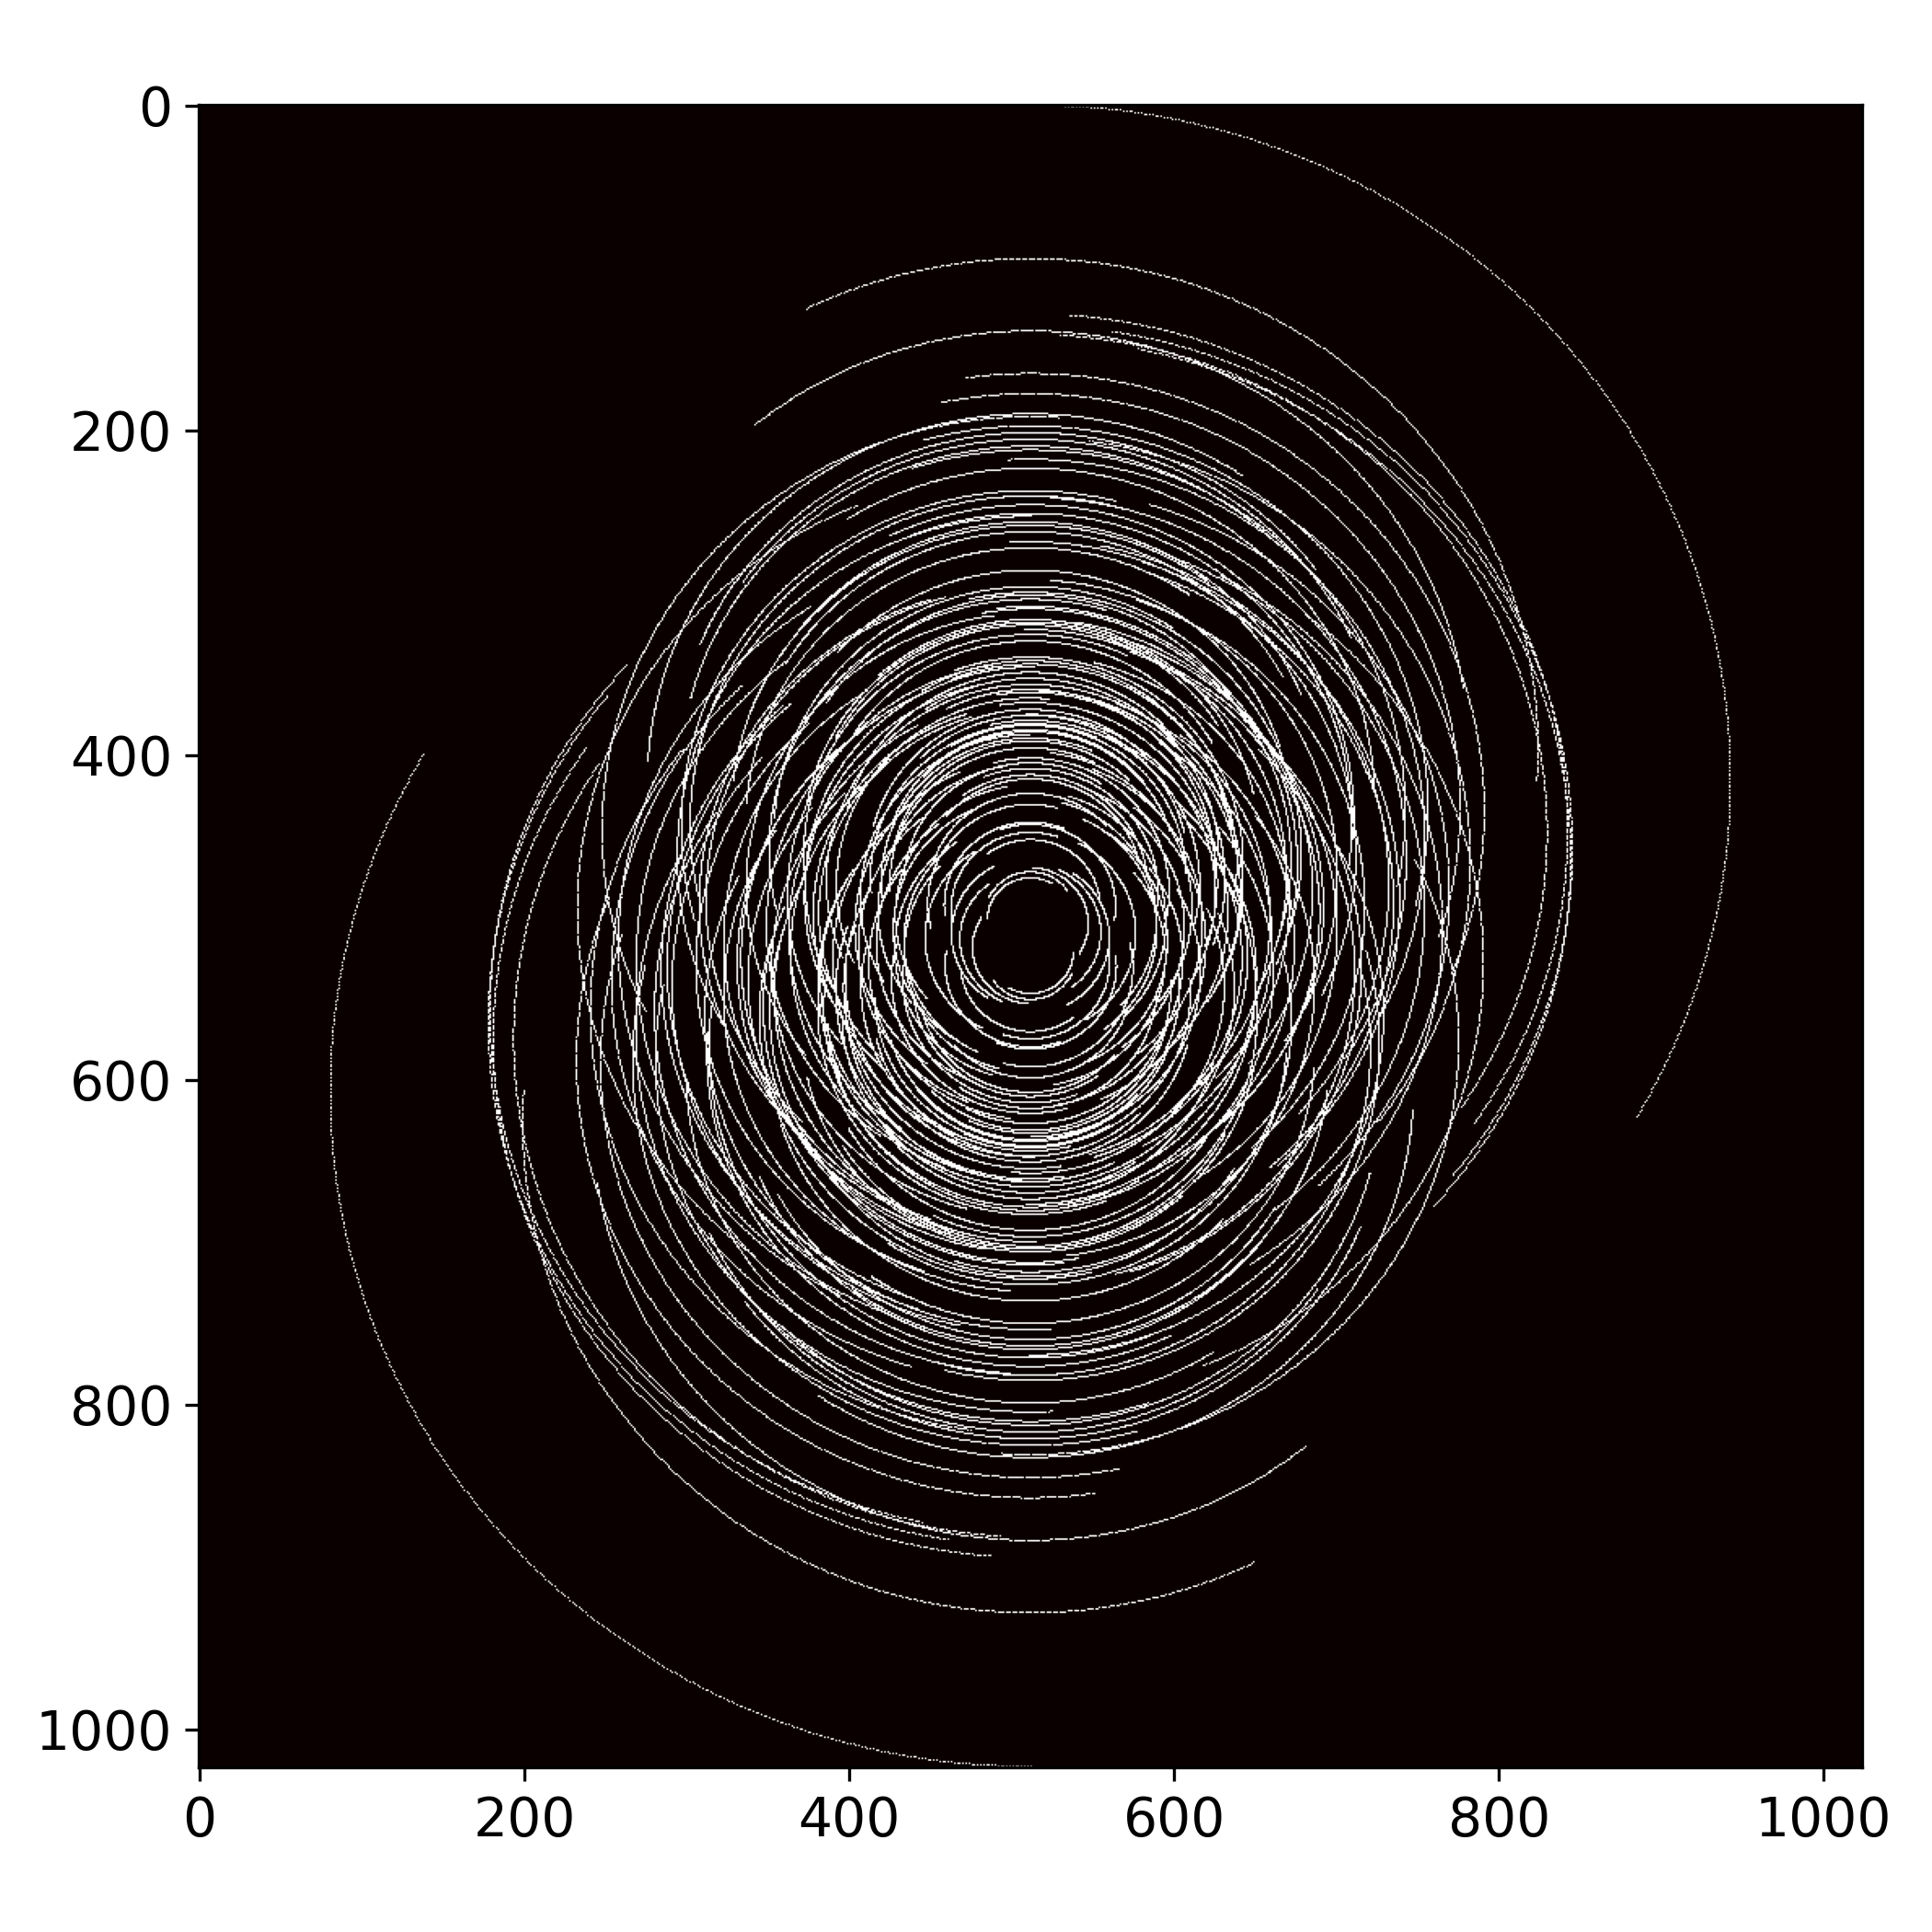
\includegraphics[width=\linewidth]{../out/sa_uv.png}
    \caption{High-resolution $uv$-coverage tracks generated by the optimal simulated annealing
             layout.}
    \label{fig:sa_uv}
\end{figure}

Visual inspection of the physical layouts reveals a striking geometric divergence between the
two search strategies. The optimal SA configuration isolates a layout with a densely
concentrated central core of antennas surrounded by a sparse outer ring. The concentrated
core generates an extensive volume of short baseline vectors, which map directly to the central
region of the $uv$-plane and coincide precisely with the high-value region of the Gaussian
weighting matrix applied by the objective function. The geometric strategy is the
theoretically natural response to a centrally weighted objective: an algorithm that
successfully exploits the local landscape around short-baseline configurations will inevitably
converge on a physically clustered solution. The fact that simulated annealing discovered this
geometry through unconstrained thermodynamic search, without any explicit guidance toward
clustering, provides strong evidence of its superior capacity for fine-grained local
exploitation on this fitness landscape.

Conversely, the optimal GA configuration exhibits a more uniformly dispersed geographical
footprint across the available pad positions. The dispersed geometry generates a greater
volume of long baseline vectors, which trace extensive elliptical arcs across the outer regions
of the $uv$-plane. These outer-edge tracks contribute a large number of raw, unweighted
$uv$-plane pixels, as is visible in Figure~\ref{fig:ga_uv}. However, the dispersed baseline
geometry produces a comparatively sparse central sampling region that fails to capture the
heavily weighted core of the Gaussian mask. The total weighted fitness score is consequently
inferior despite the GA configuration achieving a larger unweighted spatial coverage area.
The result also explains why extending the genetic algorithm budget beyond 1,000 generations
would not resolve the performance gap: the stagnated population had converged on a dispersed
topology that is locally stable under intersection crossover, and the recombination operator
lacked the capacity to transition the population toward the centrally clustered geometry that
simulated annealing naturally discovered through sustained local exploitation.

Comparison of Figure~\ref{fig:ga_uv} and Figure~\ref{fig:sa_uv} makes the consequence of
these divergent physical strategies directly observable. The SA $uv$-coverage map exhibits a
substantially denser accumulation of sampled pixels in the central region of the spatial
frequency domain, consistent with the short-baseline geometry of its physical layout. The GA
$uv$-coverage map, while covering a broader total area, is visibly sparser at the centre and
denser toward the outer boundary. The Gaussian weighting matrix assigns exponentially
decaying values to these outer pixels, meaning that the additional raw coverage area
contributed by the GA layout carries negligible mathematical weight in the objective function.
The topographic analysis therefore provides a complete geometric explanation for the
quantitative superiority of simulated annealing: the algorithm identified the physically
clustered configuration that is the optimal solution for a centrally weighted spatial frequency
objective, while the evolutionary search converged prematurely on a dispersed solution that
optimises unweighted coverage at the expense of the weighted score.

To summarise, the research results section presented the empirical performance data and
demonstrated that simulated annealing significantly outperformed all genetic algorithm
variants across every evaluated metric. The convergence analysis identified premature
stagnation as the primary limitation of the evolutionary configurations, attributing it to the
destructive effect of intersection crossover on geometric antenna sub-pairings, and
demonstrated that neither reduced selection pressure, aggressive fitness sharing, nor elevated
mutation rates resolved this limitation. The statistical analysis confirmed the superiority of
simulated annealing with a $p$-value of $1.88445 \times 10^{-11}$, eleven orders of magnitude
below the significance threshold, while simultaneously and decisively invalidating the
diversity maintenance hypothesis. Finally, the topographic analysis linked the numerical
advantage of simulated annealing to its discovery of a physically clustered antenna geometry
that constitutes the theoretically optimal response to a Gaussian-weighted spatial frequency
objective.

\section{Conclusion}

The study investigated the discrete selection of 16 antennas from the 64 MeerKAT pads to maximise 
central $uv$-coverage. A baseline genetic algorithm (GA), three genetic algorithm variants, and a simulated annealing (SA) approach 
were evaluated across 30 runs using the same Gaussian-weighted objective. 

The main finding was clear: SA consistently outperformed all GA configurations and did so 
by a statistically significant margin ($p = 1.88445 \times 10^{-11}$). The GA variants did not 
recover performance through reduced selection pressure, fitness sharing, or higher mutation. 
Instead, the GA variants tended to stagnate, indicating that the intersection crossover operator disrupted 
the spatial antenna relationships needed for high central density.

The qualitative results reinforced the interpretation. The best SA solution formed a compact 
central cluster that aligned naturally with the Gaussian weighting, while the GA solutions 
remained more dispersed and therefore underweighted in the core. The contrast underlined 
the importance of operator and landscape alignment. Population diversity alone cannot compensate 
for recombination operators that fail to preserve the spatial structures that the objective 
function rewards.

The assignment yielded several important insights into the relationship between algorithm 
design and problem landscape topology. The most significant lesson was that operator 
choice is not a secondary concern: the intersection crossover operator, while elegant in 
preserving the cardinality constraint, proved fundamentally misaligned with the geometric 
structure of the objective function. The result highlights that metaheuristic performance cannot 
be evaluated in isolation from the problem domain. Additionally, the experiment demonstrated 
that diversity mechanisms such as fitness sharing are only beneficial when the fitness 
landscape contains multiple well-separated optima of comparable quality. When the global 
optimum lies in a single clustered region, as in this case, diversity enforcement actively 
hinders convergence. Finally, the study reinforced the value of statistical rigour: without 
the 30-run sampling and Mann-Whitney analysis, the consistent superiority of simulated 
annealing could have been attributed to a fortunate initialisation rather than a structural 
algorithmic advantage.

Future work should test alternative crossover or repair operators designed to preserve 
geometric neighbourhoods, and repeat the comparison under a flat $uv$ weighting to assess 
how the ranking changes when central density is not prioritised.

\section{Acronyms}
\begin{itemize}
    \item ERAS: Earth Rotation Aperture Synthesis
    \item GA: Genetic Algorithm
    \item PSF: Point Spread Function
    \item SA: Simulated Annealing
    \item UV: Spatial frequency coordinates in the Fourier domain
\end{itemize}

\section{Symbols}
\begin{itemize}
    \item $\alpha$: significance level threshold
    \item $C$: number of unique antenna configurations
    \item $D$: aperture diameter
    \item $\Delta f$: change in fitness
    \item $H_0$: null hypothesis
    \item $H_1$: alternative hypothesis
    \item $I(l,m)$: sky brightness distribution
    \item $k$: number of active antennas
    \item $\lambda$: observation wavelength
    \item $n$: number of available antenna pads
    \item $P$: Metropolis acceptance probability
    \item $p$: calculated $p$-value
    \item $T$: system temperature
    \item $\theta$: angular resolution
    \item $u, v$: spatial frequency coordinates
    \item $V(u,v)$: complex visibility function
\end{itemize}


\begin{thebibliography}{9}

\bibitem{bremermann1962}
H. J. Bremermann, ``Optimization through evolution and recombination,'' in \emph{Self-Organizing Systems}, M. C. Yovits, G. T. Jacobi, and G. D. Goldstein, Eds. Washington, DC, USA: Spartan Books, 1962, pp. 93--106.

\bibitem{engelbrecht2007}
A. P. Engelbrecht, \emph{Computational Intelligence: An Introduction}, 2nd ed. Chichester, U.K.: John Wiley \& Sons, 2007.

\bibitem{thompson2017}
A. R. Thompson, J. M. Moran, and G. W. Swenson Jr., \emph{Interferometry and Synthesis in Radio Astronomy}, 3rd ed. Cham, Switzerland: Springer, 2017.


\end{thebibliography}

\end{document}